% 'draft' mode can be used to speed up compilation
\documentclass[final]{hcmut-report}
\usepackage{codespace}

% Draft watermark
% https://github.com/callegar/LaTeX-draftwatermark

% Encodings
\usepackage{gensymb,textcomp}

% Better tables
% Wide tables go to https://tex.stackexchange.com/q/332902
\usepackage{array,longtable,multicol,multirow,siunitx,tabularx}

% Better enum
\usepackage{enumitem}

% Graphics
\usepackage{caption,float}

% Add options for figures, like max width, framing, etc.
\usepackage[export]{adjustbox}

% References
% Use \Cref{} instead of \ref{}
\usepackage[nameinlink]{cleveref}

% FOR DEMONSTRATION PURPOSES, REMOVE IN PRODUCTION
\usepackage{mwe}

% Sub-preambles
% https://github.com/MartinScharrer/standalone


% Configurations
\coursename{Software Engineering}
\reporttype{Assignment}
\title{Smart Student Printing Service}
\advisor{& Trương Thị Thái Minh &}
\stuname{%
  & Hồ Công Gia Bảo  & 2152414 \\
  & Vũ Lê Bình & 2152440 \\
  & Võ Việt Hoàng & 2152355 \\
  & Trần Trường Giang  & 2152534 \\
  & Nguyễn Phúc Toàn  & 2153902 \\
  & Phương Xương Thịnh  & 2012479 \\
  & Nguyễn Nhất Huy  & 2053042 \\
}

% Allow page breaks inside align* environment
%\allowdisplaybreaks{}

% Makes a lot of things blue, avoid at all costs
%\everymath{\color{blue}}

% Set depth of numbering for counters
\AtBeginDocument{\counterwithin{lstlisting}{section}}

% Rename some sections
%\AtBeginDocument{\renewcommand*{\contentsname}{Contents}}
%\AtBeginDocument{\renewcommand*{\refname}{References}}
%\AtBeginDocument{\renewcommand*{\bibname}{References}}

% Custom commands
%\newcommand*\mean[1]{\bar{#1}}

\begin{document}
\coverpage%

\tableofcontents
\listoffigures
\listoftables

\pagebreak

\section{Member list \& Workload}

\

\begin{table}[H]
\begin{tabular}{|l|l|l|l|}
\hline
\textbf{No.} & \textbf{Full Name} & \textbf{Work Assignment}                                                                                                                                   & \textbf{Contribution} \\ \hline
1            & Võ Việt Hoàng      & \begin{tabular}[c]{@{}l@{}}- User Requirement and Domain Context\\ - Use case diagrams and tables\\ - Architecture diagrams\\ - MVP Wireframe\end{tabular} & 100\%                 \\ \hline
2            & Phương Xương Thịnh & \begin{tabular}[c]{@{}l@{}}- User Requirement\\ - Draw and describe use cases\\ - Draw component diagram\\ - General Editing and Finalization\end{tabular} & 100\%                 \\ \hline
3            & Nguyễn Phúc Toàn   & \begin{tabular}[c]{@{}l@{}}- User Requirement\\ - Draw and describe use cases\\ - Draw class diagram\\ - Draw activity diagram\\ - General Editing and Finalization\end{tabular}     & 100\%                 \\ \hline
4            & Hồ Công Gia Bảo    & \begin{tabular}[c]{@{}l@{}}- User Requirement\\ - Draw sequence diagram\\ - General Editing and Finalization\end{tabular}                                  & 100\%                 \\ \hline
5            & Trần Trường Giang  & \begin{tabular}[c]{@{}l@{}}- User Requirement\\ - Draw class diagram\end{tabular}                                                                          & 100\%                 \\ \hline
6            & Nguyễn Nhất Huy    & \begin{tabular}[c]{@{}l@{}}- User Requirement\\ - Use case diagrams and tables\\ - Draw sequence diagram\\ - General Editing and Finalization\end{tabular} & 100\%                 \\ \hline
7            & Vũ Lê Bình         & \begin{tabular}[c]{@{}l@{}}- Draw Activity Diagram\\ - General Editing and Finalization\end{tabular}                                                       & 100\%                 \\ \hline
\end{tabular}
\end{table}

\clearpage

\section{Project Description}

\subsection{Describe project}

The university is intent to build a Student Smart Printing Service (HCMUT\_SSPS) for serving
students in its campuses to print their documents.\\

The system consists of some printers around the campuses. Each printer has ID,
brand/manufacturer name, printer model, short description, and the location (campus name,
building name, and room number).\\

The system allows a student to print a document by uploading a document file onto the system,
choose a printer, and specifying the printing properties such as paper size, pages (of the file) to be printed, one-/double-sided, number of copies, etc. The permitted file types are limitted and configured by the Student Printing Service Officer (SPSO). \\

The system has to log the printing actions for all students, including student ID, printer ID, file
name, printing start and end time, number of pages for each page size. \\

The system allows the SPSO to view the printing history (log) of all students or a student for a
time period (date to date) and for all or some printers. Of course, a student can also view his/her
printing log for a time period together with a summary of number of printed pages for each
page size. \\

For each semester, the university give each student a default number of A4-size pages for
printing. Students are allowed to buy some more using the feature Buy Printing Pages of the
system and pay the amount through some online payment system like the BKPay system of the
university. The system only allow a student to print some number of pages when it does not
exceed his/her account (page) balance. Note that, one A3 page is equivalent to two A4 pages.
The SPSO has a feature to manage printers such as add/enable/disable a printer.\\

The SPSO also has a feature to manage other configuration of the system such as changing the
default number of pages, the dates that the system will give the default number of pages to all
students, the permitted file types accepted by the system.\\

The reports of the using of the printing system are generated automatically at the end of each
month and each year and are stored in the system, and can be viewed by the SPSO anytime.
All users have to be authenticated by the HCMUT\_SSO authentication service before using the
system.\\

The system is provided through a web-based app or a mobile app.

\subsection{Domain Context}

\subsubsection{Overview}

HCMUT\_SSPS is a comprehensive system for university student document printing. It includes printers, user authentication, printing management, page quotas, online payments, configuration tools, and usage reports.

\subsubsection{Actors and Roles}

Students use the system to print, purchase pages, and view history. The SPSO administers printers, settings, and reports.

\subsubsection{Key Concepts and Interactions}

Printers have IDs, brands, models, and locations. Print jobs include file details and printing preferences. Printing history tracks past jobs. Page quotas manage A4 page limits. Online payments expand quotas. System settings configure behavior. Usage reports summarize activity.

\subsubsection{Domain Rules}

Students authenticate via HCMUT\_SSO. File types are controlled by the SPSO. Page quotas reset each semester. Overusing quotas is restricted. A3 pages count as two A4 pages. SPSO manages printers and settings. Reports are auto-generated.

\subsubsection{Domain Events}

Upload initiates printing. Print job submission requests printing. Completion marks success. Purchasing adds pages. Monthly/yearly reports offer insights. SPSO's actions affect printers and settings.

\subsubsection{Relationships}

Students are linked to quotas and history. Print jobs connect students, printers, and preferences. Reports summarize all activity. SPSO manages printers and settings for system effectiveness.


\subsection{Stakeholders and their current needs}
\begin{itemize}
\item \textbf{Students (Users):} Primary users of the system. They utilize the Student Smart Printing Service (HCMUT\_SSPS) to print documents, manage their page balance, and view printing history.

\item \textbf{Student Printing Service Officer (SPSO):} The SPSO administers the system, managing printers, configuration settings, and viewing printing logs and reports.
\item \textbf{HCMUT Administration:} Responsible for overseeing the efficient provision of the printing service to students. They make decisions regarding resource allocation and service enhancements based on usage trends.

\item \textbf{HCMUT IT Department:} Ensures the secure setup and integration of the smart printing service within the university network. They are responsible for integrating with existing systems such as HCMUT\_SSO.

\item \textbf{Printers:} The physical devices located around campus, each with a unique ID, brand, model, description, and specific location details, including campus name, building name, and room number. They play a central role in the printing process.

\item \textbf{BKPay System:} The online payment system integrated into the Student Smart Printing Service for purchasing additional printing pages. It facilitates financial transactions related to printing.

\item \textbf{System Database:} The database within the system is responsible for storing data, including printing history, reports, user information, and configuration settings. It ensures data integrity and accessibility.

\item \textbf{HCMUT\_SSO Authentication Service}: The authentication service that verifies user identities before granting access to the Student Smart Printing Service. It ensures secure user authentication.

\item \textbf{Web-Based and Mobile Apps:} The delivery channels through which users access the system. They provide the user interface for interacting with the printing service.

\item \textbf{Reports:} Automated reports generated by the system at the end of each month and year. They summarize printing usage data and provide insights for stakeholders.

\end{itemize}

\subsection{Benefits of HCMUT-SSPS for each stakeholder}

\subsubsection{Students (Users):}
\begin{itemize}
\item \textbf{Convenience:} HCMUT-SSPS offers students a convenient and user-friendly way to print documents from both web and mobile apps. This convenience can improve their overall experience and productivity on campus.
Choice and Customization: Students benefit from the ability to choose printers based on their preferences and specific requirements. This customization ensures that their printing needs are met efficiently. (Source: Journal of Computing Sciences in Colleges - Student Smart Printing: An Approach to Mobile and Secure Printing)
\item \textbf{Transparency:} Access to their printing history and page balance allows students to monitor and manage their printing resources effectively. They can make informed decisions about when and how to use their allocated pages.
\end{itemize}
\subsubsection{Student Printing Service Officer (SPSO):}
\begin{itemize}
\item \textbf{Efficient Printer Management:} SPSO benefits from efficient printer management capabilities, including adding, enabling, or disabling printers. This streamlines the maintenance and operation of the printing service.
\item \textbf{Configuration Control:} The ability to configure system settings such as default page limits and permitted file types allows SPSO to tailor the printing service to the university's specific requirements and policies. (Source: International Journal of Computer Applications - Secure Printing System for Students in Universities)
\item \textbf{Usage Insights:} Viewing printing history logs and generating reports provides valuable insights into system usage. This data helps in optimizing resource allocation and planning future upgrades.

\end{itemize}
\subsubsection{HCMUT Administration:}
\begin{itemize}
\item \textbf{Resource Management:} HCMUT-SSPS facilitates effective resource management by providing usage trends and reports. Administrators can make data-driven decisions regarding resource allocation, reducing waste and cost.
\item \textbf{Enhanced Service:} The system enables the administration to offer an efficient and modern printing service to students, improving the overall quality of services provided on campus.
\end{itemize}
\subsubsection{HCMUT IT Department:}
\begin{itemize}
\item \textbf{Secure Integration:} The IT Department benefits from the secure integration of HCMUT-SSPS with existing university systems like HCMUT\_SSO and BKPay. This ensures data security and compatibility.
\item \textbf{Network Efficiency:} By securely setting up the smart printing service within the university network, the IT Department can ensure that the system operates efficiently without compromising network performance.
\end{itemize}

\clearpage
\section{Project Requirements}

\subsection{Functional Requirements}

\subsubsection{For Students}
\begin{itemize}
\item \textbf{Document Printing:} The system must allow a student to initiate the printing of a document by uploading a supported document file format (e.g., PDF, DOCX).
\item \textbf{Printer Selection:} The student should have the ability to select a specific printer from the available options.
\item \textbf{Printing Properties:} The student must specify various printing properties, including paper size (e.g., A4, A3), the range of pages to be printed (e.g., pages 1-5), single-sided or double-sided printing, and the number of copies.
\item \textbf{View Printing History:} Students must have access to their printing history, which provides a record of past print jobs. This history should include details such as the timestamp of each print job, the total number of pages printed, and the name of the printer used.
\item \textbf{User Authentication:} To access the printing service, students must log in using the HCMUT\_SSO authentication service. Users who are not logged in should not be able to use the service.
\item \textbf{Page Balance Purchase:} Students should be able to purchase additional page balance using the BKPay system, allowing them to print more pages. The updated page balance should be reflected immediately in the application.
\item \textbf{Page Balance Notification:} If a student's page balance is depleted, the printing functionality must be temporarily disabled. Users should receive a prominent notification offering the option to purchase more page balance.
\end{itemize}

\subsubsection{For Student Printing Service Officer}
\begin{itemize}
\item \textbf{View Printing History:} The SPSO must have the ability to access the printing history of all students or specific students within a specified time period. Each log entry should include details such as the number of pages printed, the printer used, and student information.
\item \textbf{System Configuration:} The SPSO should have the authority to modify system configurations, including default page counts, accepted file types, and other settings that govern the behavior of the printing service.
\item \textbf{Printer Management:} The SPSO should be able to manage printers, including adding new printers, enabling or disabling existing printers, and configuring printer-specific settings.
\item \textbf{User Information Access:} The SPSO must be able to access detailed user information, including balance, name, and student ID.
\item \textbf{Report Generation:} The service must automatically generate and store monthly and yearly reports summarizing page usage, the number of students using the service, and comparisons with previous time intervals.
\end{itemize}

\subsubsection{For HCMUT Administrator}
\begin{itemize}
\item \textbf{User Account Management:} The administrator must have the capability to create, redefine, deactivate, or delete user accounts, including those of students and SPSOs.
\item \textbf{Payment History Access:} The administrator should be able to access and review the payment history of each student account at any time.
\item \textbf{Report Access:} The administrator should have access to monthly and yearly reports detailing page usage and student statistics compared to previous intervals.
\end{itemize}

\subsection{Non-Functional Requirements}

\subsubsection{For Students}
\begin{itemize}
\item \textbf{Data Privacy:} Uploaded files by students should be securely accessible only by the student who uploaded them or the Student Printing Service Officer.
\item \textbf{User Interface Responsiveness:} The user interface should load within 5 seconds to ensure a smooth and responsive experience when interacting with buttons and inputs.
\item \textbf{Server Performance:} The application server must remain accessible and responsive even when handling up to 50 concurrent student uploads.
\item \textbf{Page Count Accuracy:} The system must accurately count or calculate the number of pages printed by each student.
\end{itemize}

\subsubsection{For Student Printing Service Officer}
\begin{itemize}
\item \textbf{Comprehensive Documentation:} A detailed document must accompany the application, explaining its operation and providing step-by-step instructions for actions such as enabling/disabling printers, configuring printer page limits, specifying permitted file types, and viewing logs.
\item \textbf{Configuration Propagation:} When the SPSO updates printing configurations (e.g., default page limits or paper size), the changes must be applied to all printers across the network within 1 minute.
\end{itemize}

\subsubsection{For HCMUT Administrator}
\begin{itemize}
\item \textbf{Account Management Efficiency:} Any changes made to user accounts by the administrator (e.g., creation, redefinition, deactivation, deletion) should be completed by the system within 10 minutes.
\end{itemize}

\clearpage
\section{Overall use cases}

\begin{figure}[H]
  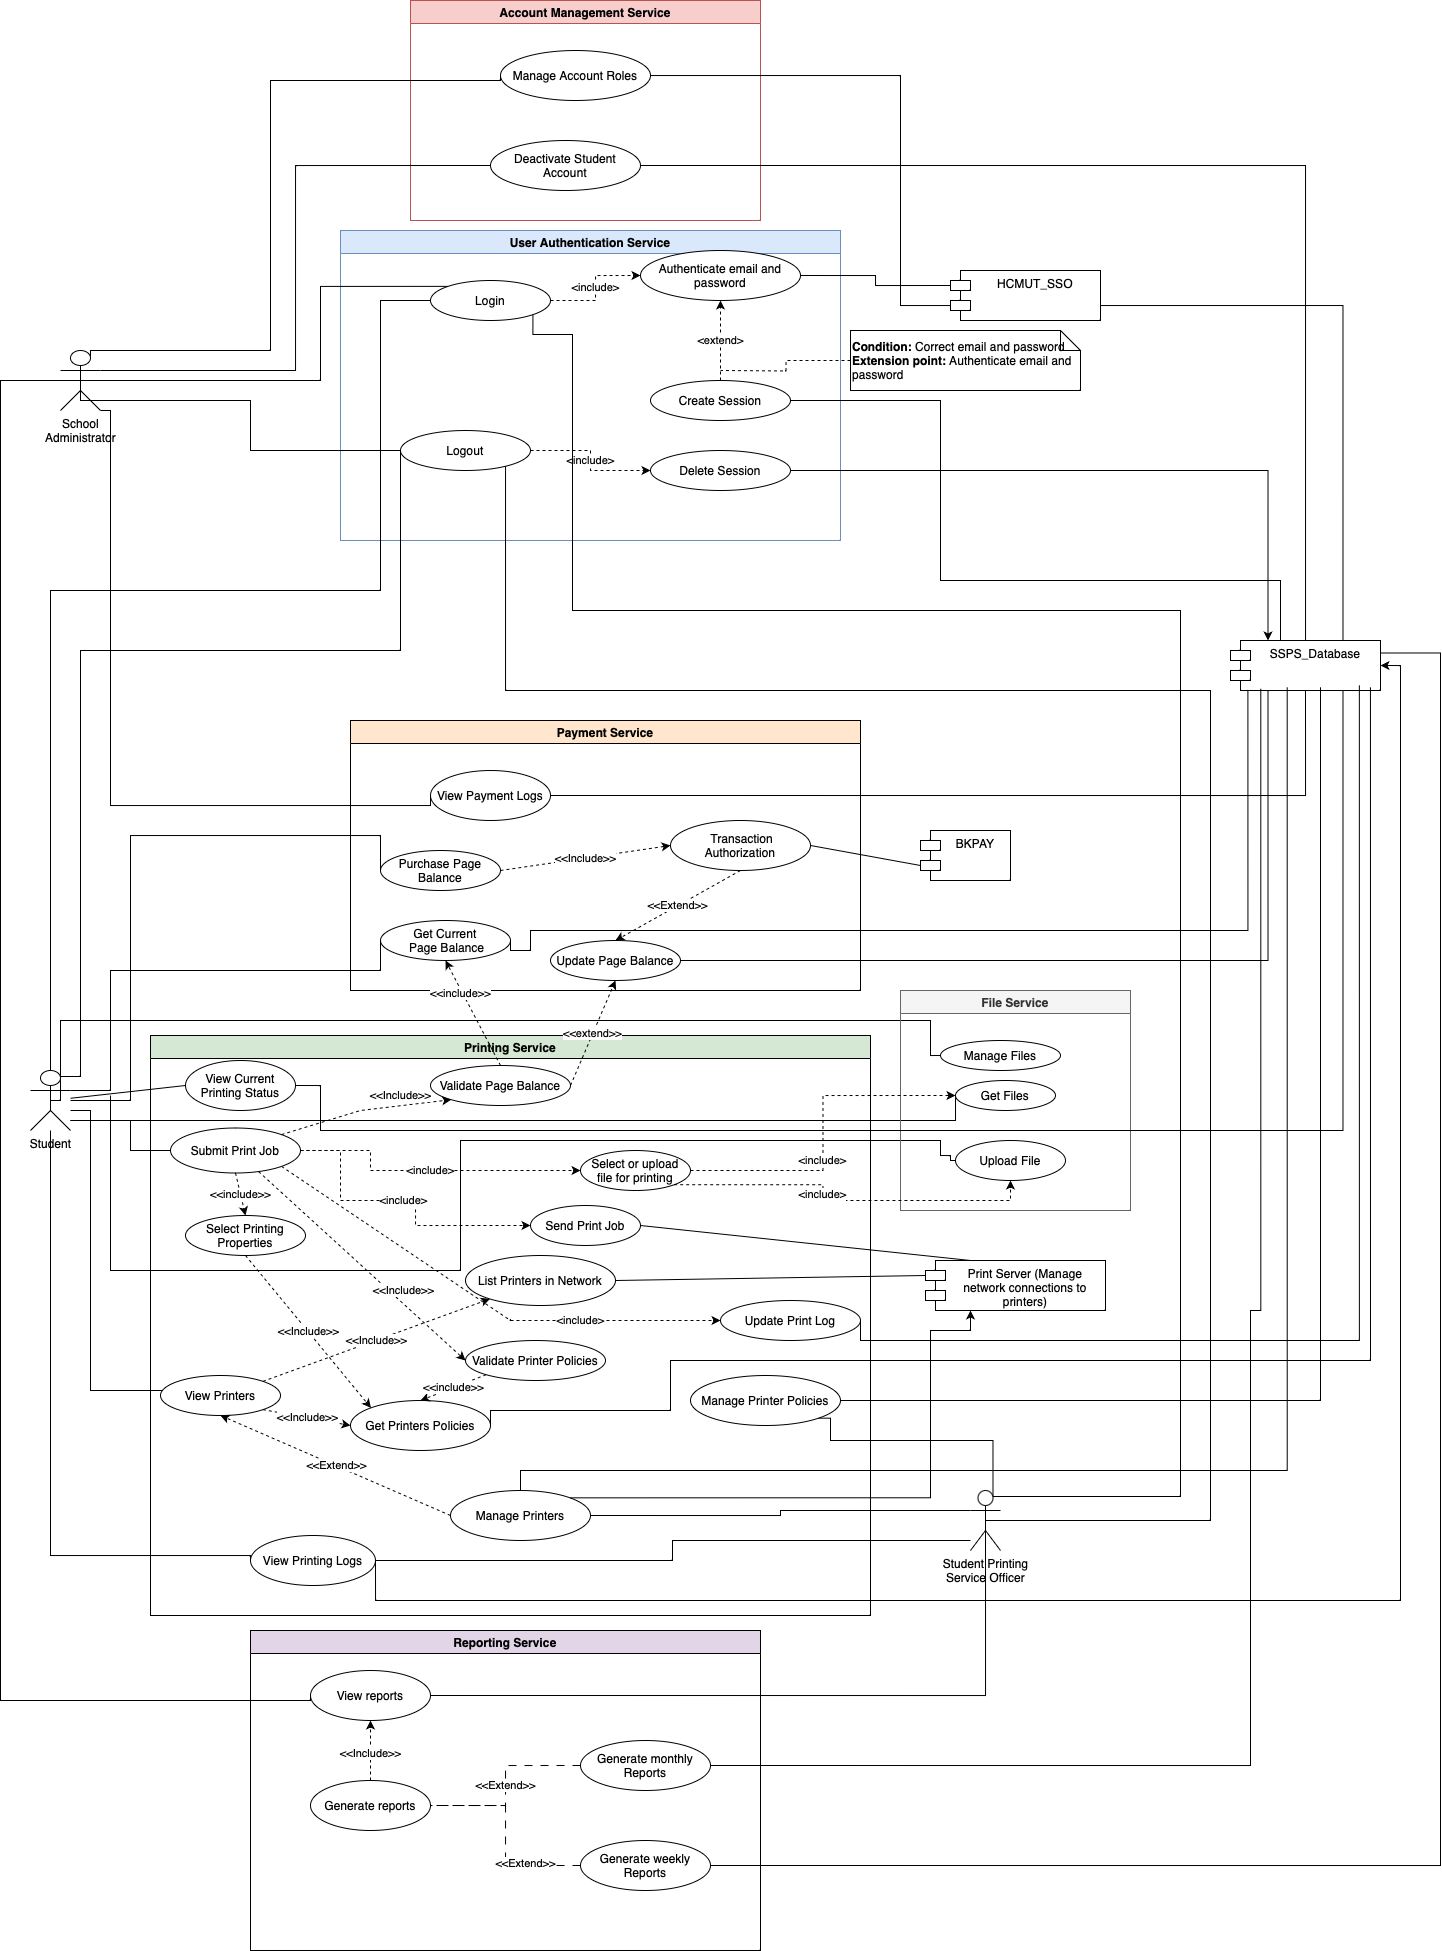
\includegraphics[max width=0.9\linewidth]{chapters/3. use-case-diagram/overall-use-case-diagram.png}
  \caption{Use case of the whole system}%
\end{figure}

\

For the full diagram, check out the following links: \href{https://drive.google.com/file/d/1WRi-N7SIQ2TsGwEkwdd48GqCGhodFedc/view?usp=drive_link}{Draw.io diagram}, \href{https://drive.google.com/file/d/1CZHHrL5VMrCAE1oMELBysDtHTPctMH6j/view?usp=drive_link}{Full resolution image}.

\

The whole system of SmartStudentPrintingService contains 5 modules:

\begin{itemize}
\item \textbf{Account Management Service:} This module is responsible for managing user accounts within the system, specifically catering to the administrative functions. It allows administrators to create, redefine, deactivate, or delete user accounts, including those of students and Student Printing Service Officers (SPSOs).

\item \textbf{User Authentication Service:} The User Authentication Service ensures secure access to the system by verifying the identity of users. It utilizes the HCMUT\_SSO authentication service to authenticate students and other users before granting access to the system's features.

\item \textbf{Payment Service:} This module facilitates online payments for students to purchase additional printing pages. It integrates with payment systems like BKPay, allowing students to extend their page balance for printing. The service ensures that purchased page balances are reflected immediately within the application.

\item \textbf{Printing Service:} The Printing Service is a core component that enables students to initiate and manage print jobs. It handles the upload and printing of documents, printer selection, specifying printing properties (e.g., paper size, page range), and maintaining a history of printing actions. It also enforces page balance checks and notifications when balance is depleted.

\item \textbf{File Service:} The File Service is responsible for securely handling and storing uploaded document files by students. It ensures that files are accessible only to the respective student who uploaded them and authorized personnel, such as SPSOs. This module plays a crucial role in maintaining data privacy and security.

\item \textbf{Reporting Service:} The Reporting Service automatically generates and stores reports summarizing system usage. It compiles statistics on page usage, the number of students using the service, and provides comparisons with previous time intervals (monthly and yearly). These reports are valuable for assessing resource utilization and making informed decisions about the printing service.
\end{itemize}

\section{Detailed use cases}

\subsection{User Authentication and Session Management Use Cases}

\subsubsection{Use-case diagram}

\begin{figure}[H]
  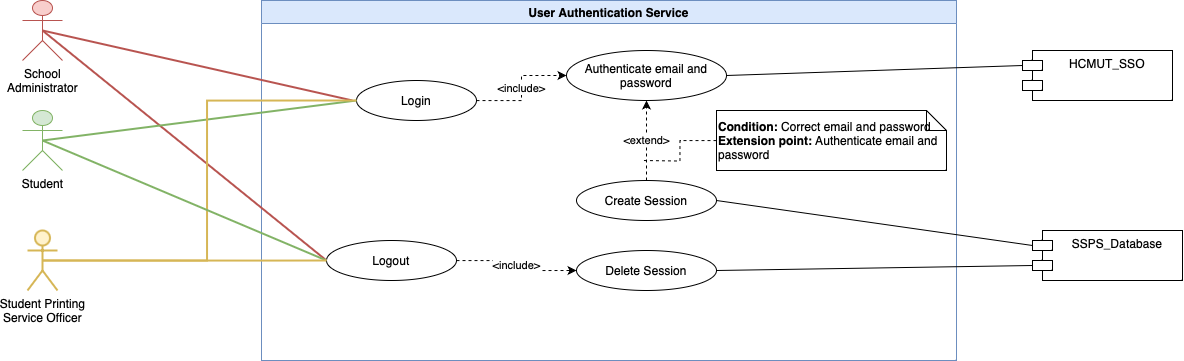
\includegraphics[max width=0.9\linewidth]{chapters/3. use-case-diagram/authentication-use-case-diagram.png}
  \caption{Use case of the whole system}%
\end{figure}

\subsubsection{Table format: Login Feature}

\begin{table}[H]
\begin{tabular}{|p{5cm}|p{9cm}|}
\hline
\textbf{Use Case Name} & User Login and Session Management \\
\hline
\textbf{Actors} & Student User, HCMUT\_SSO, User Authentication Service, SSPS\_Database \\
\hline
\textbf{Description} & Allows a registered user to log in and maintain a user session. \\
\hline
\textbf{Trigger} & User clicks on the Login button on the navbar. \\
\hline
\textbf{Preconditions} & The system is running and accessible. The user has valid HCMUT\_SSO credentials. \\
\hline
\textbf{Postconditions} & User is logged in, and a user session is created in SSPS\_Database. \\
\hline
\textbf{Normal Flows} & 
1. User get redirected to HCMUT\_SSO for authentication. \\
&2. User enters HCMUT\_SSO username and password on the HCMUT\_SSO login page. \\
&3. HCMUT\_SSO authenticates user credentials and redirects back to SSPS upon successful login. \\
&4. SSPS creates a user session. \\
&5. User gains access to system features. \\
\hline
\textbf{Exceptions} & 
From 2a. If the user's HCMUT\_SSO credentials are invalid, display an error message. \\
&From 3a. If the user cancels the login on the HCMUT\_SSO page, display an error message and do not create a user session. \\
\hline
\end{tabular}
\caption{User Login and Session Management Use Case}
\end{table}

\subsubsection{Table Format: Logout Feature}

\begin{table}[H]
\begin{tabular}{|p{5cm}|p{9cm}|}
\hline
\textbf{Use Case Name} & User Logout and Session Termination \\
\hline
\textbf{Actors} & Student User, User Authentication Service, SSPS\_Database \\
\hline
\textbf{Description} & Allows a registered user to log out and terminate their user session. \\
\hline
\textbf{Trigger} & User clicks on the user avatar on navbar and click on the "Logout" button. \\
\hline
\textbf{Preconditions} & User is logged in with an active user session. \\
\hline
\textbf{Postconditions} & User is logged out, and the user session is removed from SSPS\_Database. \\
\hline
\textbf{Normal Flows} & 
1. System terminates the user's session. \\
&2. User is logged out and no longer has access to system features. \\
\hline
\textbf{Exceptions} & None \\
\hline
\end{tabular}
\caption{User Logout and Session Termination Use Case}
\end{table}

\subsection{Submit Printing Job and Printer Management}

\subsubsection{Use-case diagram}

\begin{figure}[H]
  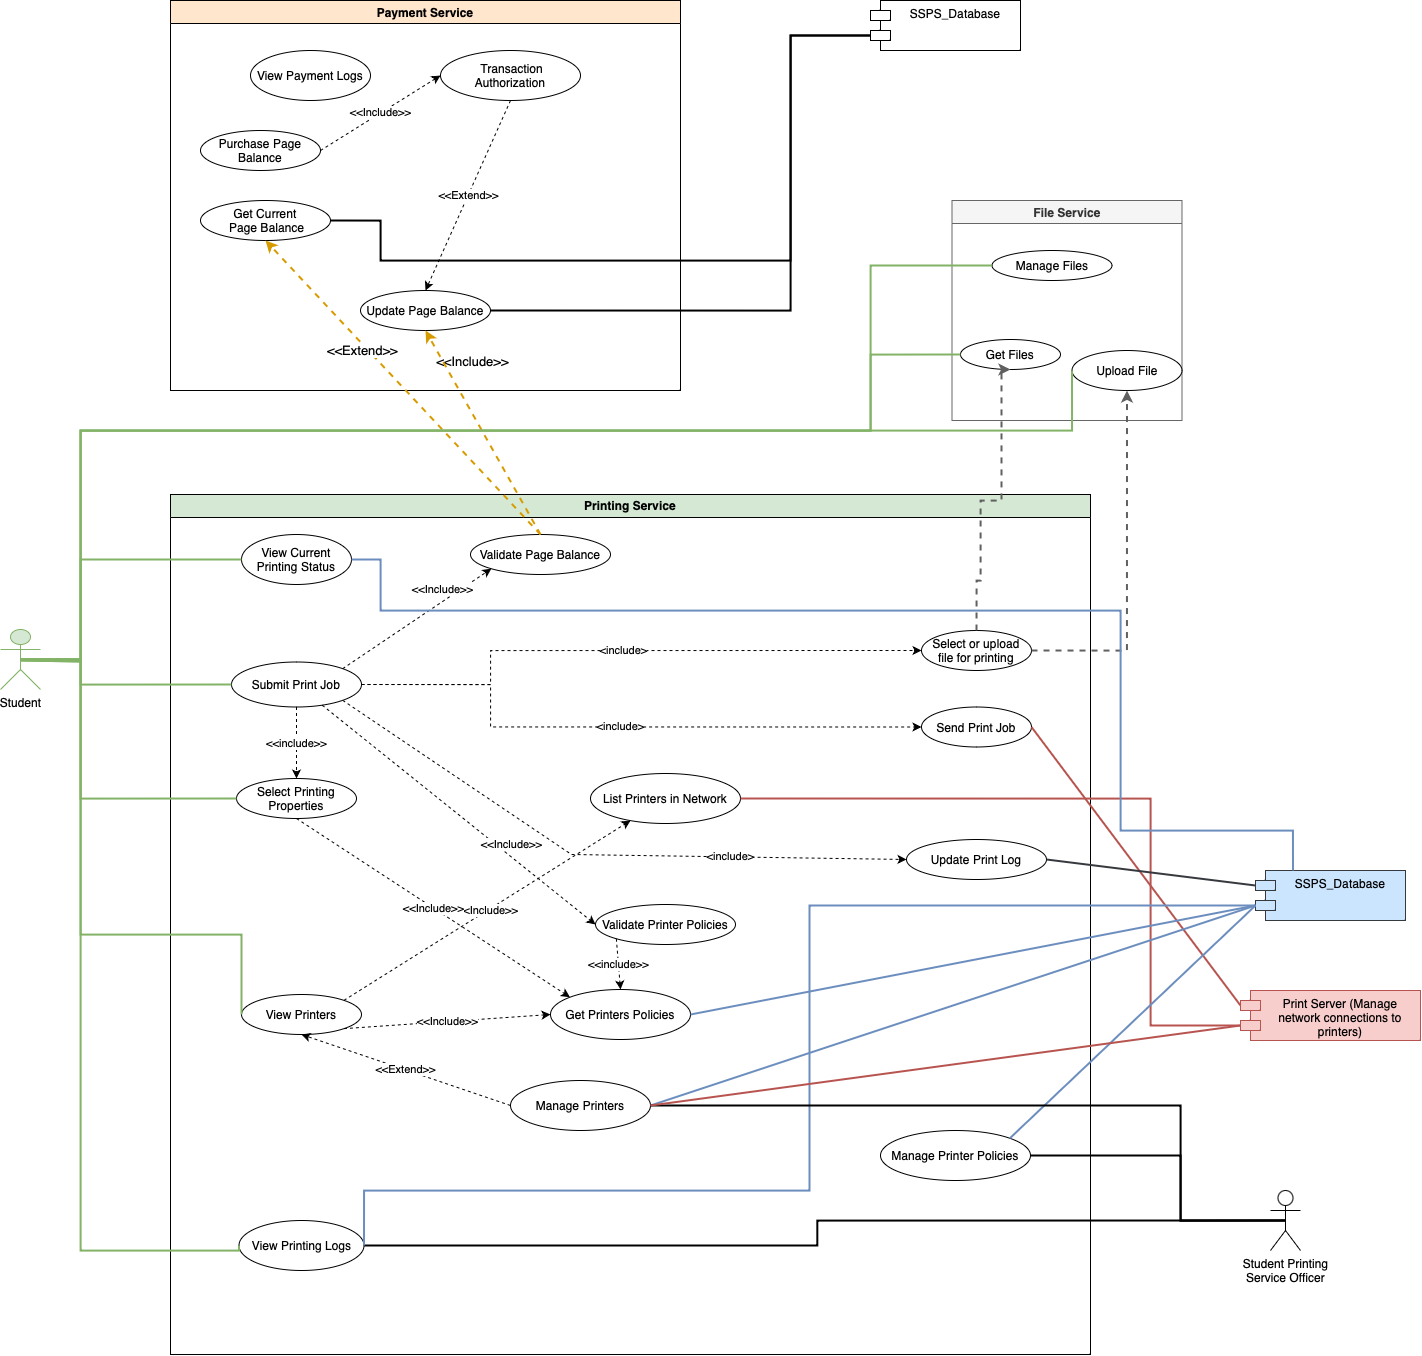
\includegraphics[max width=0.9\linewidth]{chapters/3. use-case-diagram/printing-use-case-diagram.png}
  \caption{Use case of the whole system}%
\end{figure}

\subsubsection{Table Format: Submit Print Job}

\begin{table}[H]
\begin{tabular}{|p{5cm}|p{9cm}|}
\hline
\textbf{Use Case Name} & Submit Print Job \\
\hline
\textbf{Actors} & Student User, Printing Service, Print Server, Payment Service, SSPS\_Database \\
\hline
\textbf{Description} & SPSO generates detailed reports at the end of each month and year, including total printed pages, page size breakdown, printer activity, student-specific logs, purchased pages summary, and system configuration changes. \\
\hline
\textbf{Trigger} & User clicks on "+ New Print" button on the sidebar  \\
\hline
\textbf{Preconditions} & User is logged in with an active user session. The document to be printed is uploaded and accessible. \\
\hline
\textbf{Postconditions} & The print job is successfully submitted for processing, and the user is notified when the print job is completed. \\
\hline
\textbf{Normal Flows} & 
1. User selects the desired printer for the print job. \\
&2. User selects the document to be printed. \\
&3. User specifies printing properties such as paper size, single-/double-sided, number of copies, and other preferences. \\
&4. User confirms the print job submission. \\
&5. System processes the print job and adds it to the print queue. \\
&6. User receives a confirmation message that the print job has been successfully submitted. \\
&7. User is notified when the print job is completed. \\
\hline
\end{tabular}
\caption{Submit Print Job}
\end{table}

\begin{table}[H]
\begin{tabular}{|p{5cm}|p{9cm}|}
\hline
\textbf{Alternative Flows} & 
\textbf{From 2a.} User clicks on Uploaded Files tab: \\
&2a.1. User clicks on their uploaded file from the list. \\
&2a.2. Proceed with step 3 and onwards as in the normal flow. \\
& \textbf{From 2b.} User clicks on Integrations tab: \\
&2b.1. User clicks on the integration button (e.g., Google Drive, OneDrive). \\
&2b.2. User follows the integration flow to select a file. \\
&2b.3. Proceed with step 3 and onwards as in the normal flow. \\
& \textbf{From 7b.} If the user runs out of page balance and chooses the Get More Balance button: \\
&7b.1. User clicks the "Get More Balance" button. \\
&7b.2. User is redirected to the page for adding more balance to their account. \\
&7b.3. Proceed with the balance addition process. \\
&7b.4. After successfully adding more balance, return to the print job confirmation step (step 4) and continue with the normal flow. \\
\hline
\textbf{Exceptions} & 
\textbf{From 5a.} If the selected printer is unavailable or offline, display an error message and allow the user to choose an alternative printer. \\
& \textbf{From 7a.} If the user runs out of page balance and chooses Cancel, display a notification and do not proceed with printing. \\
\hline
\end{tabular}
\caption{Submit Print Job (cont.)}
\end{table}

\subsection{Report Generation and Viewing}

\begin{figure}[H]
  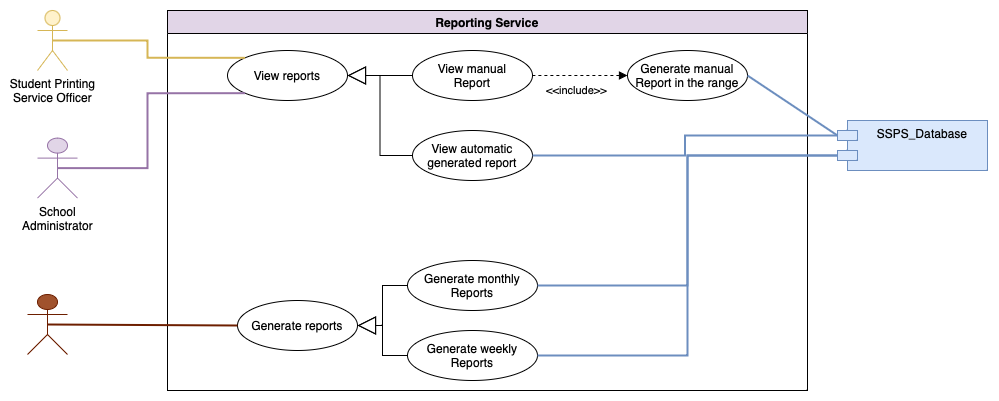
\includegraphics[max width=0.9\linewidth]{chapters/3. use-case-diagram/reporting-service.png}
  \caption{Use case of the whole system}%
\end{figure}

\subsubsection{Table Format: Generate Report}

\begin{table}[H]
\begin{tabular}{|p{5cm}|p{9cm}|}
\hline
\textbf{Use Case Name} & Report Generation \\
\hline
\textbf{Actors} & Student Printing Service Officer, School admin, Cron-job module, SSPS\_Database, Reporting Service \\
\hline
\textbf{Description} & SPSO generates detailed reports either on-demand by selecting a time range or through automated generation triggered by a cron job module. Reports include total printed pages, page size breakdown, printer activity, student-specific logs, purchased pages summary, and system configuration changes. \\
\hline
\textbf{Trigger} & - End of each month and year for automated generation. \\
& - SPSO is logged in and navigates to Report page and clicks on "Generate Report". \\
\hline
\textbf{Preconditions} & 1. SPSO is logged into the system. \\
& 2. For on-demand generation, SPSO selects "Reports" link from the sidebar. \\
\hline
\textbf{Postconditions} & 1. Reports for the specified time period are generated and stored. \\
\hline
\textbf{Normal Flows} & 1. "Generate Report" dialog is opened \\
& 2. SPSO selects the time range and report type. \\
& 3. SPSO initiates report generation. \\
& 4. The system generates and stores the report. \\
& 5. SPSO views and downloads the report. \\
\hline
\end{tabular}
\caption{Report Generation}
\end{table}

\begin{table}[H]
\begin{tabular}{|p{5cm}|p{9cm}|}
\hline
\textbf{Alternative Flows} & \textbf{From 1.} Cron job module triggers the generation of weekly and monthly reports. \\
& 1.1. The system generates and stores reports. \\
& 1.2. SPSO can access these reports at any time. \\
\hline
\textbf{Exceptions} & 1. If SPSO is not logged in, on-demand generation cannot proceed. \\
& 2. If no data is available for the specified time period, an empty report may be generated for on-demand or automated generation. \\
\hline
\end{tabular}
\caption{Report Generation (cont.)}
\end{table}

\subsubsection{Table Format: Report Viewing}

\begin{table}[H]
\begin{tabular}{|p{5cm}|p{9cm}|}
\hline
\textbf{Use Case Name} & View reports \\
\hline
\textbf{Actors} & Student Printing Service Officer, School admin, SSPS\_Database, Reporting Service\\
\hline
\textbf{Description} & Viewing the printing report \\
\hline
\textbf{Trigger} &SPSO navigates to Report page. \\
\hline
\textbf{Preconditions} & User is logged in with an active user session. User either has school administrator or SPSO role. \\
\hline
\textbf{Postconditions} & None \\
\hline
\textbf{Normal Flows} &1. The system find and list all reports from the database.\\
&2. The user selects one of the report link from the list.\\
&3. A dialog is shown and the user can view the rendered report \\
\hline
\textbf{Alternative Flows} & \textbf{From 1.} User clicks on Generate Report Manually button.\\
&1.2 User select the desired time range of the report.\\
&1.3 The report is then generated using the data got from the database.\\
&1.4 Continue from Step 3. in Normal Flows \\
&  \textbf{From 3.} User clicks on Download Report \\
&  3.1 The report is downloaded to the user device \\
\hline

\end{tabular}
\caption{View reports}
\end{table}
\clearpage
\section{Activity Diagram}

\subsection{Printing service}
\begin{figure}[H]
\centering
  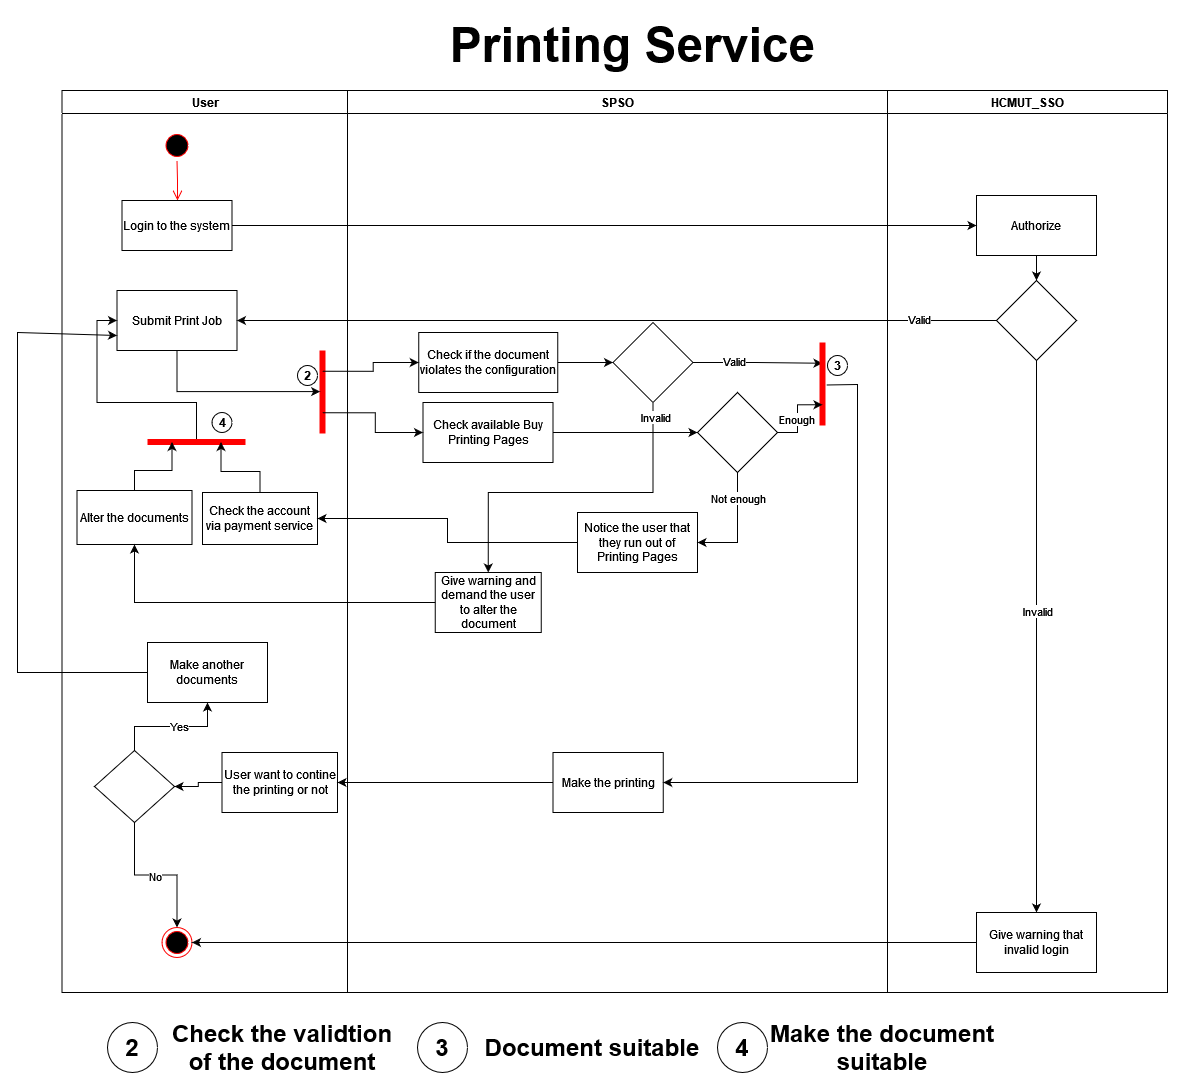
\includegraphics[max width=0.9\linewidth,origin = c]{chapters/4. system-modeling/activity/activity_printing.drawio.png}
  \caption{Activity diagram for Printing Service}%
\end{figure}

The printing service demonstrates the steps involved in producing printed documents. Initially, the user accesses the system by logging in through HCMUT\_SSO, which involves an authorization process. Once the user successfully logs into the website, they gain the ability to upload their documents for printing. At this point, the SPSO conducts two checks: it assesses the document's configuration and verifies the available remaining printing pages, akin to a "bank account" for printing. If any problems are identified during these checks, the user is notified and can make necessary adjustments before the printing process is finalized.

\subsection{View account status}

\begin{figure}[H]
\centering
  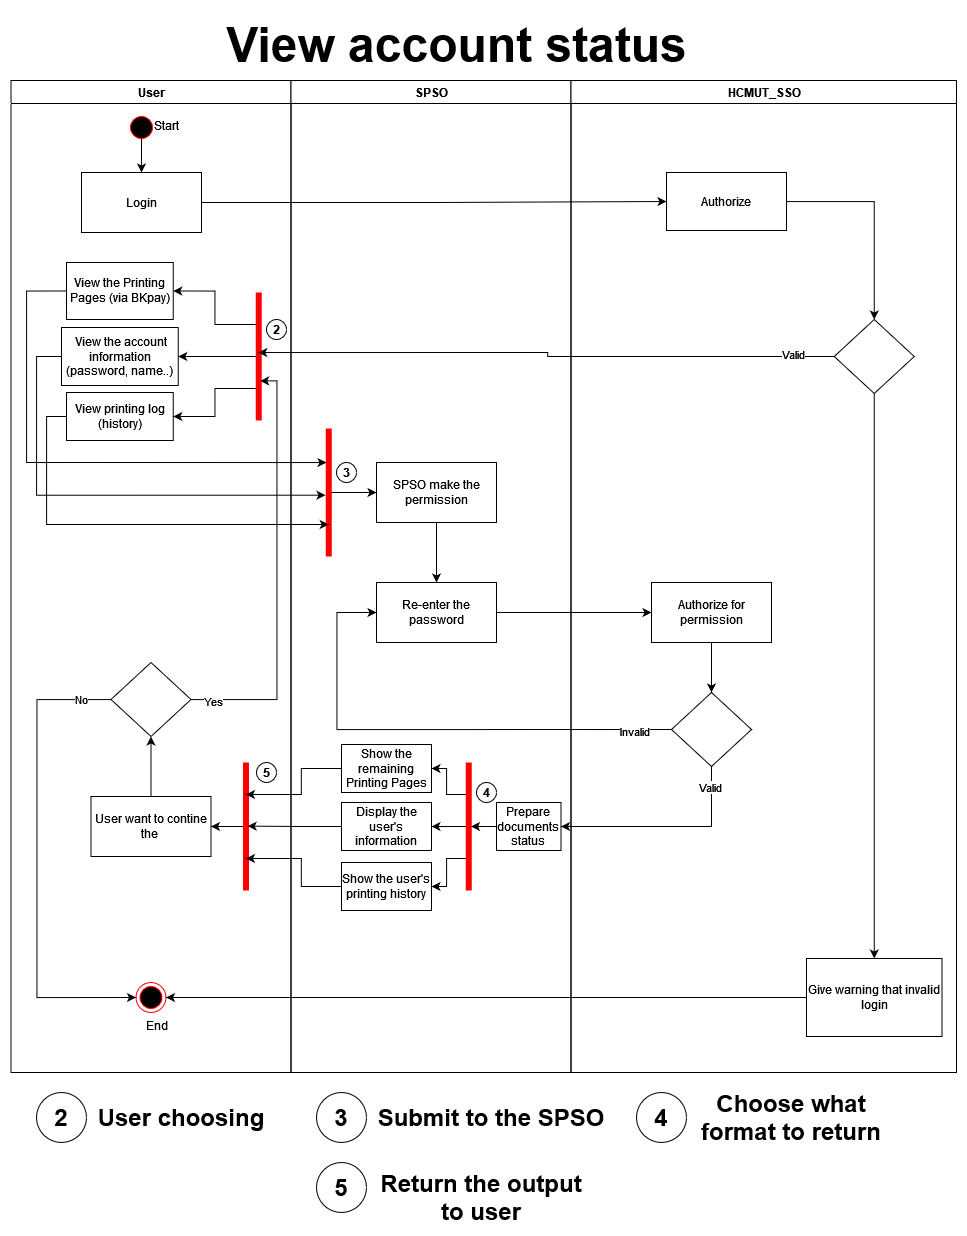
\includegraphics[max width=0.9\linewidth,origin = c]{chapters/4. system-modeling/activity/view account_acitivty.png}
  \caption{Activity diagram for View account status}%
\end{figure}

The "View account status" use-case enables users to access their personal account information, which includes their "bank account" balance, personal details, and printing history. Upon logging into the system via HCMUT\_SSO, users can request this information from the system. The SPSO (System for Printing Services and Operations) is responsible for generating the requested data and displaying it to the user. It's worth noting that users are required to re-enter their password before making the request to SPSO.

\subsection{Payment Service}

\begin{figure}[H]
\centering
  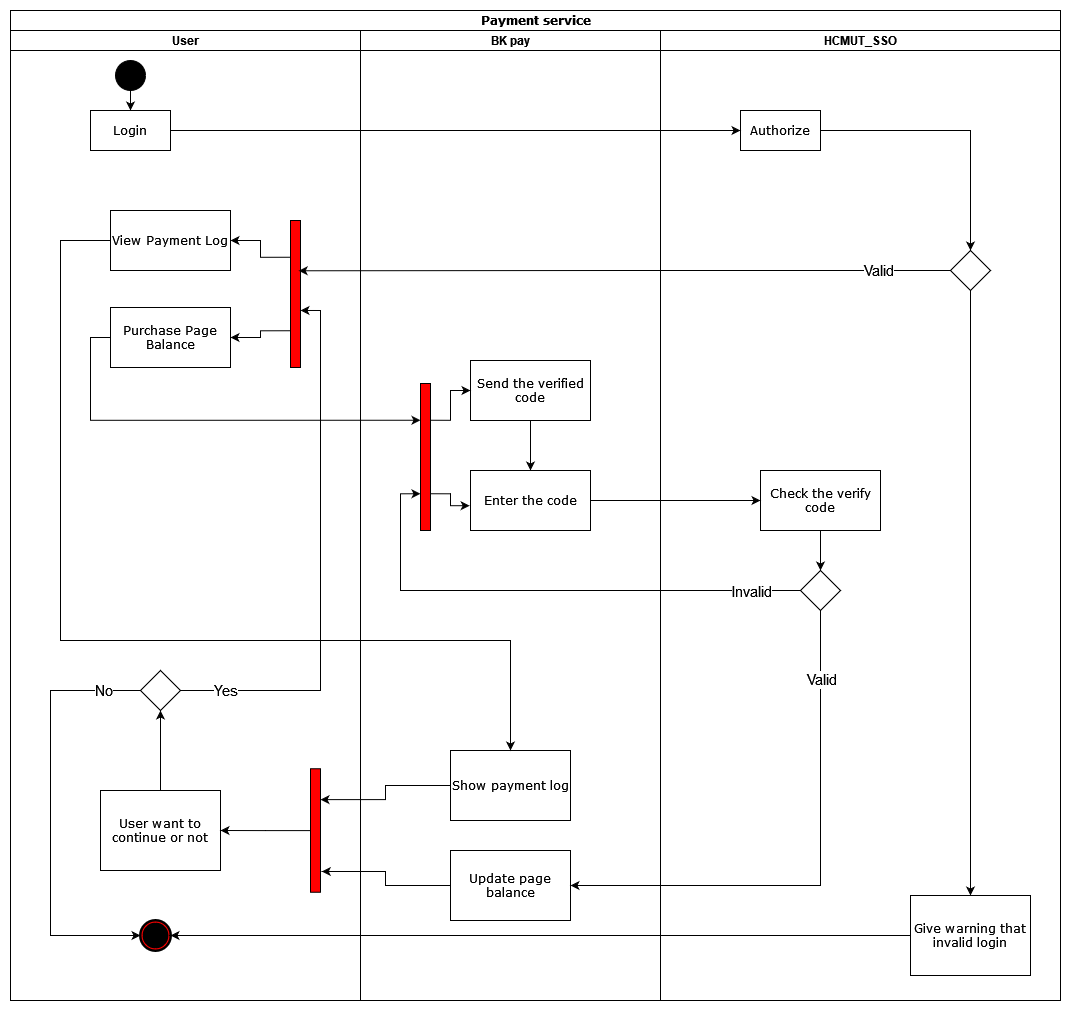
\includegraphics[max width=0.9\linewidth,origin = c]{chapters/4. system-modeling/activity/Activity_payment.png}
  \caption{Activity diagram for Payment Service}%
\end{figure}

The payment service allows students to purchase the balance and the school administrator can view the payment log. Initially, the user accesses the system by logging in through HCMUT\_SSO, which involves an authorization process. When logging into the system via HCMUT\_SSO, students can request the BKpay to purchase their balance. In order to purchase, students have to verify their transaction by receiving and entering the correct code. Students can request to resend the code if they haven’t received or they want to receive a new one to enter again. After finishing the transaction, the BKpay system will update the current balance for students.

\subsection{Report Service}

\begin{figure}[H]
\centering
  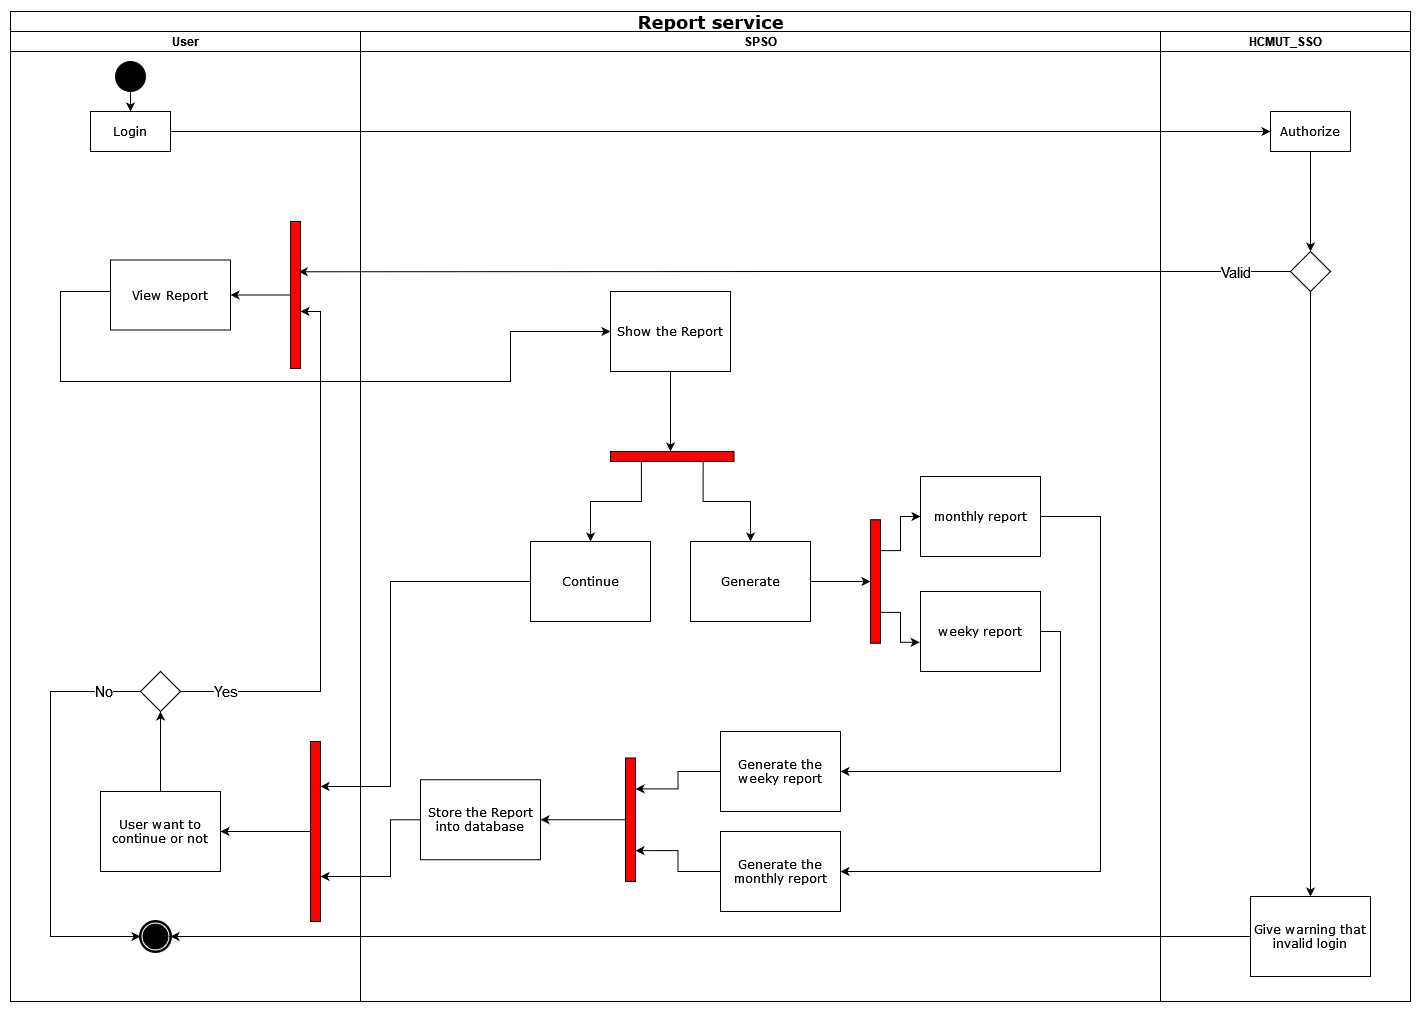
\includegraphics[max width=0.9\linewidth,origin = c]{chapters/4. system-modeling/activity/activity_report.png}
  \caption{Activity diagram for Report Service}%
\end{figure}

The report service enables users to view and generate the report. Initially, the user accesses the system by logging in through HCMUT\_SSO, which involves an authorization process. Upon logging into the system via HCMUT\_SSO, view the report from the Student Printing Service Officer. Users can request to generate the report on a weekly or monthly basis. After generate, the report will be stored into the database.












\section{Sequence Diagram}
\subsection{View Printer}                                                                        
\begin{figure}[H]
\centering
  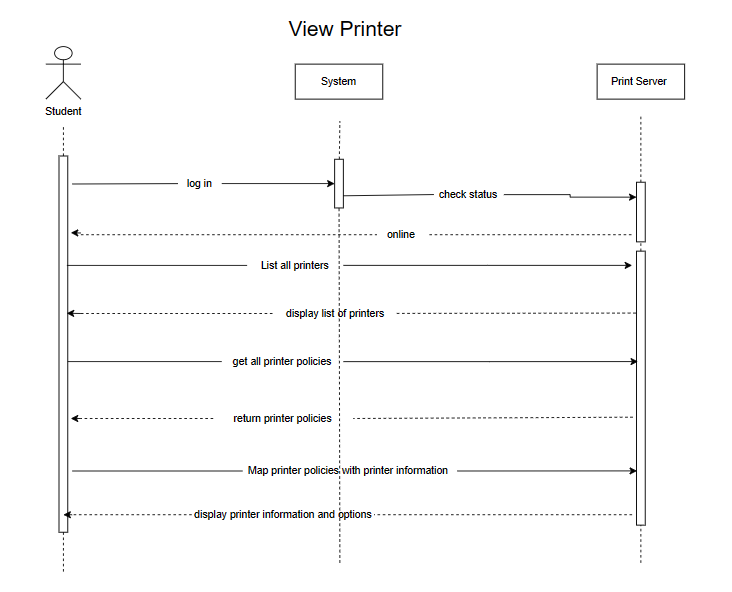
\includegraphics[max width=0.9\linewidth,origin = c]{chapters/4. system-modeling/picture/ViewPrinter.png}
  \caption{Sequence Diagram of View Printer}%
\end{figure}
Students login into the system, the system will check status in the print server and send server status (running) back to the students. The students will request to see all printers. The print server will display a list of all printers to the student. The students will request to see all printer policies. The print server will return all printer policies to the students. The server will map printer policies with printer information and display it back to students.
\subsection{View Printing Logs}
\begin{figure}[H]
\centering
  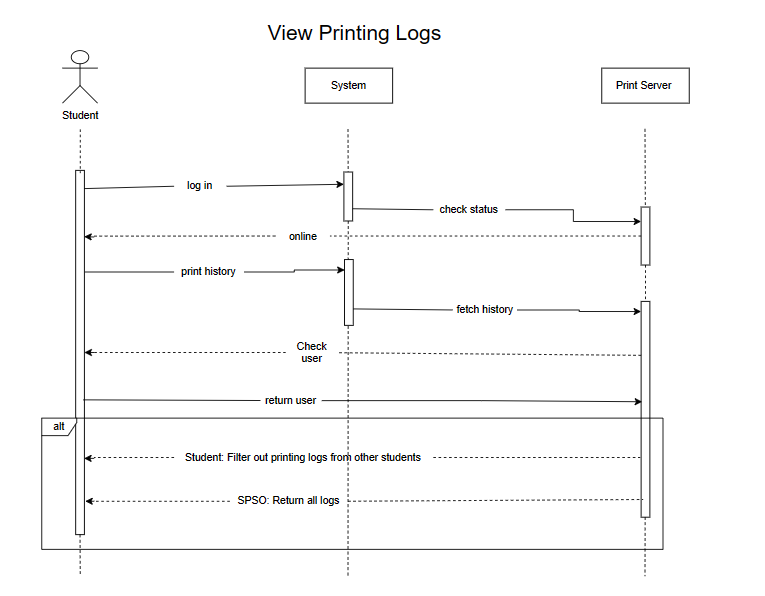
\includegraphics[max width=0.9\linewidth,origin = c]{chapters/4. system-modeling/picture/ViewPrintingLogs.png}
  \caption{Sequence Diagram of View Printing Logs}%
\end{figure}
Users login into the system, the system will check status in the print server and send server status (running) back to the students. The users send the request to print history to the system. The system will fetch the logs into the print server. The server will check the status of the user. User will return the status back to the server. If the user is a student, we will filter out printing logs from other students, if the user is Student Printing Service Officer, we will return all logs.

\subsection{Manage Printer Policies}
\begin{figure}[H]
\centering
  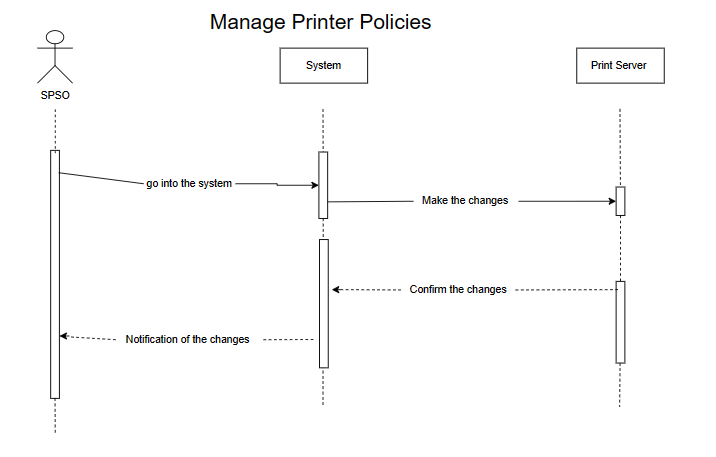
\includegraphics[max width=0.9\linewidth,origin = c]{chapters/4. system-modeling/picture/ManagePrinterPolicies.png}
  \caption{Sequence Diagram of Manage Printer Policies}%
\end{figure}
SPSO goes into the system, makes the changes in the print server. The server then will send the confirmation of the changes to the system. The system will notify the SPSO that the changes are applied.
\subsection{Log Out}
\begin{figure}[H]
\centering
  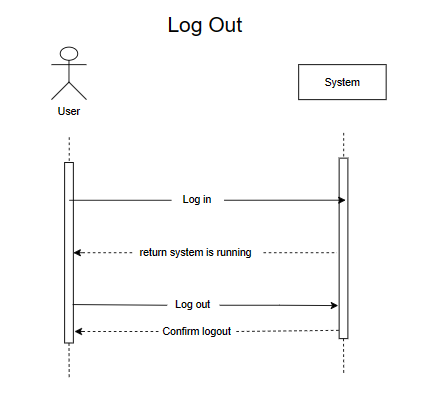
\includegraphics[max width=0.9\linewidth,origin = c]{chapters/4. system-modeling/picture/LogOut.png}
  \caption{Sequence Diagram of Log Out}%
\end{figure}
Users login into the system. The system will send server status (running) back to the users. The Users log out of the system. The system confirms the logging out.

\subsection{Submit Print Job}
\begin{figure}[H]
\centering
  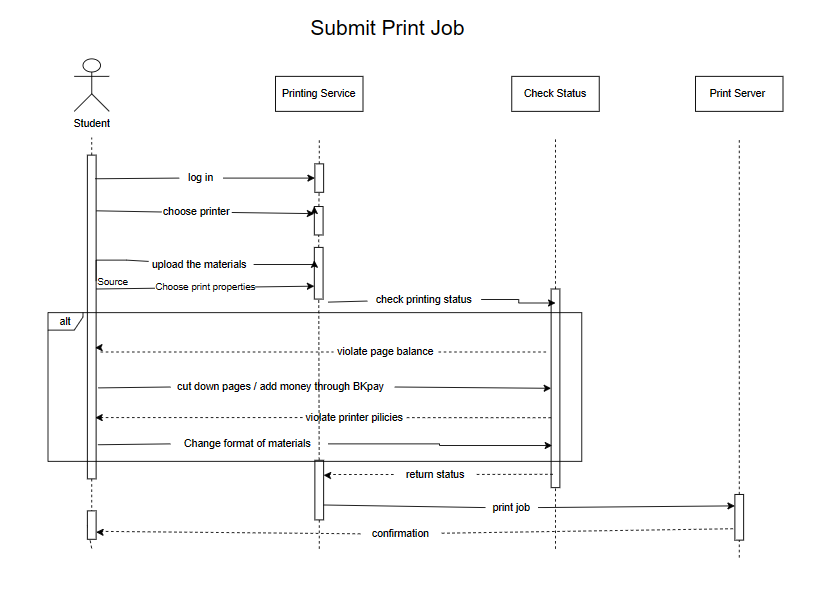
\includegraphics[max width=0.9\linewidth,origin = c]{chapters/4. system-modeling/picture/SubmitPrint.png}
  \caption{Sequence Diagram of the Submit Print Job}%
\end{figure}
Students login into the printing service, choose the printer and upload the materials. The printing service will check the status for these 2 exception flows. If it violates the page balance, students are required to cut down pages or add money through Bkpay2. If it violates the printer policies, students must change the format of the materials that meet the accepted configuration of the system. Then the status will be returned to the printing service. The submission of the print job will be sent from printing service to print server. The confirmation will be sent back to the user.

\section{Class Diagram}
\begin{figure}[H]
  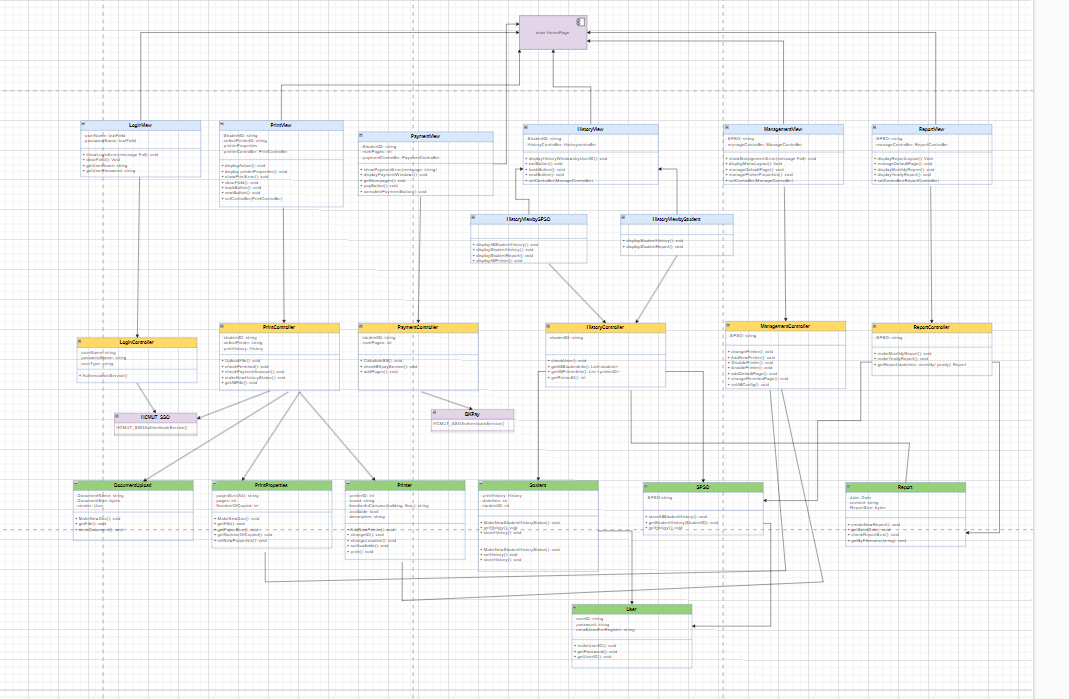
\includegraphics[max width=0.9\linewidth,origin = c]{chapters/4. system-modeling/picture/class.PNG}
  \caption{Class Diagram}%
\end{figure}

The class diagram presents a structured view of a system with classes that cover various aspects of a school management system, including printing services, payment, user history, and report generation. Notably, there is a \textbf{LoginView} class that likely handles user authentication, which is connected to a \textbf{LoginController}. There's an inheritance hierarchy where SPSO classes inherit from Student and User classes respectively, indicating different types of users. The \textbf{HistoryController} class is connected to two different views, suggesting that it handles the logic for displaying historical data for both staff and students. \textbf{ReportController} manages report generation, while \textbf{PaymentController} seems to deal with financial transactions. The Printer class has a composition relationship with \textbf{PrintProperties} and \textbf{DocumentUpload}, indicating that printing functionality is central to this system. Overall, the diagram suggests a comprehensive system designed to manage various administrative tasks in an educational setting.\\

Overall, The diagram illustrates a multi-faceted educational institution management system, integrating various functionalities such as authentication, printing, payment processing, and report management. It emphasizes modularity and object-oriented design, with clear divisions between user interfaces, control logic, and data models. There are specific pathways for user interaction flows and data processing, indicating a system capable of handling complex, interrelated tasks while maintaining a separation of concerns for easier maintenance and scalability.\\

For further references see \href{https://drive.google.com/file/d/15Wbk8DiISW-IV2xAhueTpo-qr4kJO3H4/view?usp=sharing}{Class Diagram on drawio}
\clearpage
\section{MVP Wireframe}

Shown below is the MVP Wireframe implemented using Figma.

The full diagram can be found in this \href{https://www.figma.com/file/Sfcv02sNfcQDcNzJZBcMjC/SE?type=design&node-id=1302-148192&mode=design}{Figma link}.

\subsection{Dashboard (Student View)}

\begin{figure}[H]
  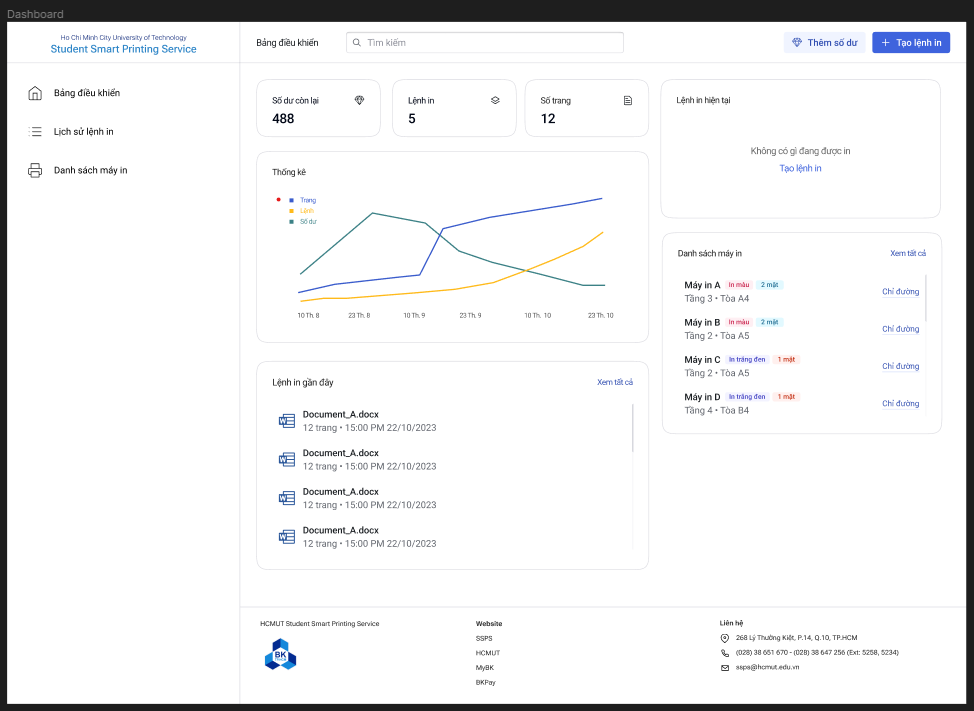
\includegraphics[max width=0.9\linewidth]{chapters/5. mvp-wireframe/1 - Dashboard.png}
  \caption{Dashboard View}%
\end{figure}

The dashboard view allows the user to have quick glance over some basic informations like the amount of balance they have left as well as some printing statistics.\

The sidebar includes links that allow the user to navigate to other features of the application.

\subsection{Create Print Job (Student View)}

From the dashboard, clicking on "Tạo lệnh in" on the top right will open the New Print dialog.

\begin{figure}[H]
  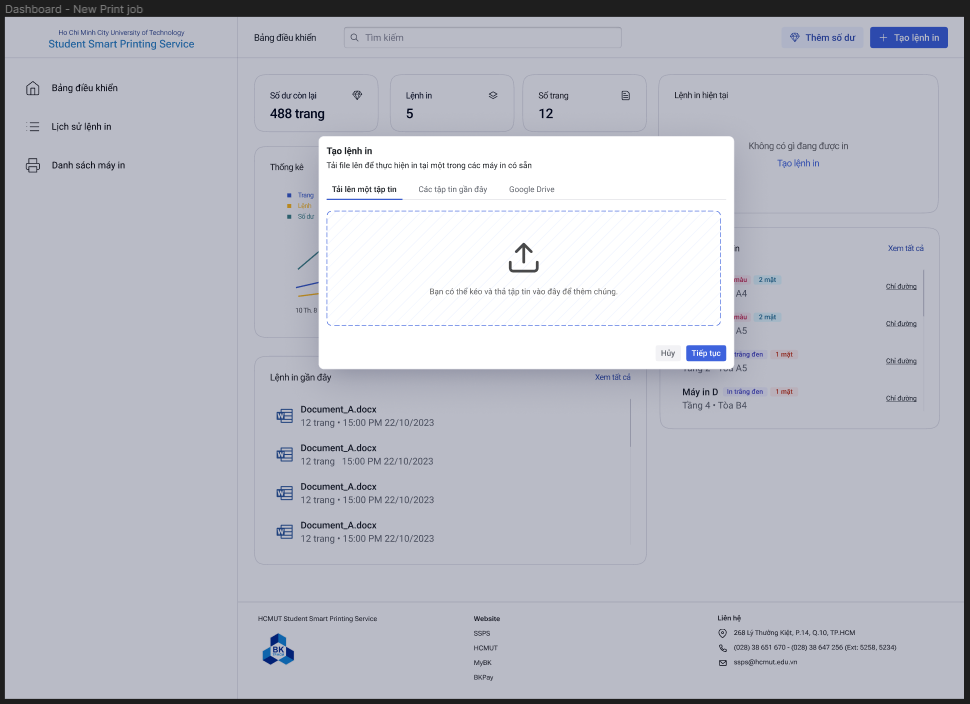
\includegraphics[max width=0.9\linewidth]{chapters/5. mvp-wireframe/2 - Dashboard - Create Print.png}
  \caption{New Print Dialog - Select File}%
\end{figure}

The user can either upload a new file, select a file from those recently uploaded, or select a file from one of the file storage provider integration (Google Drive, OneDrive, etc.).


\begin{figure}[H]
  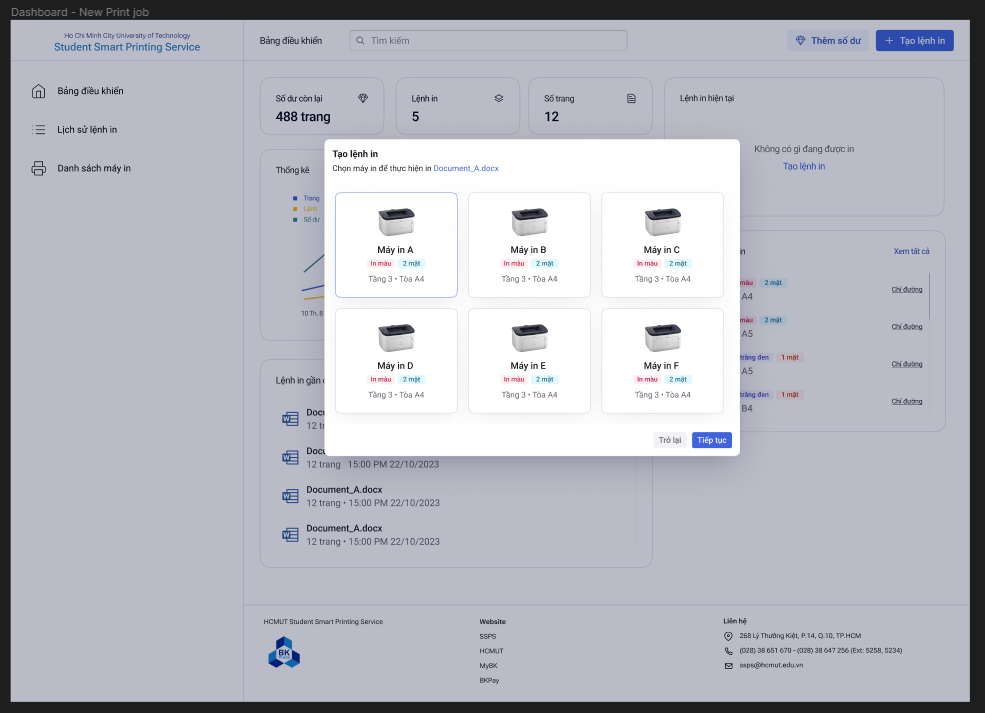
\includegraphics[max width=0.9\linewidth]{chapters/5. mvp-wireframe/3 - Dashboard - Select Printer.png}
  \caption{New Print Dialog - Select Printer}%
\end{figure}

After selecting a file, the user will need to select the printers they would like to use. Each printer card provides the user with information like the printer capabilities as well as its location.

\begin{figure}[H]
  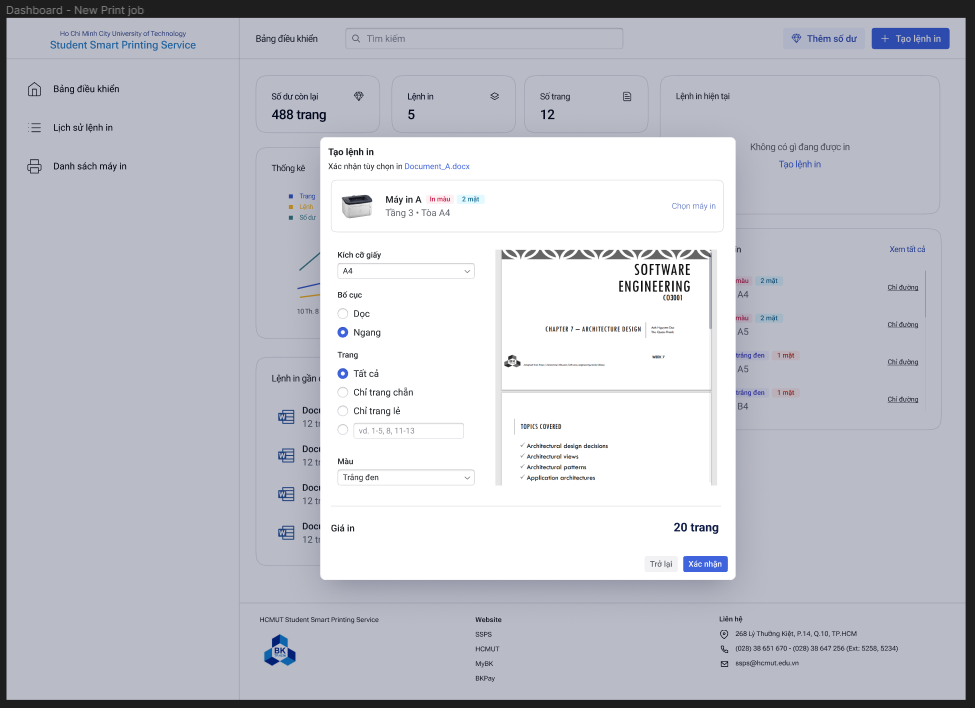
\includegraphics[max width=0.9\linewidth]{chapters/5. mvp-wireframe/4 - Dashboard - Select Properties.png}
  \caption{New Print Dialog - Select Properties}%
\end{figure}

Finally, the user will have to select the properties that they want their file to be printed. The available options will be affected by the configuration of the selected printers.

\subsection{Print History}

\begin{figure}[H]
  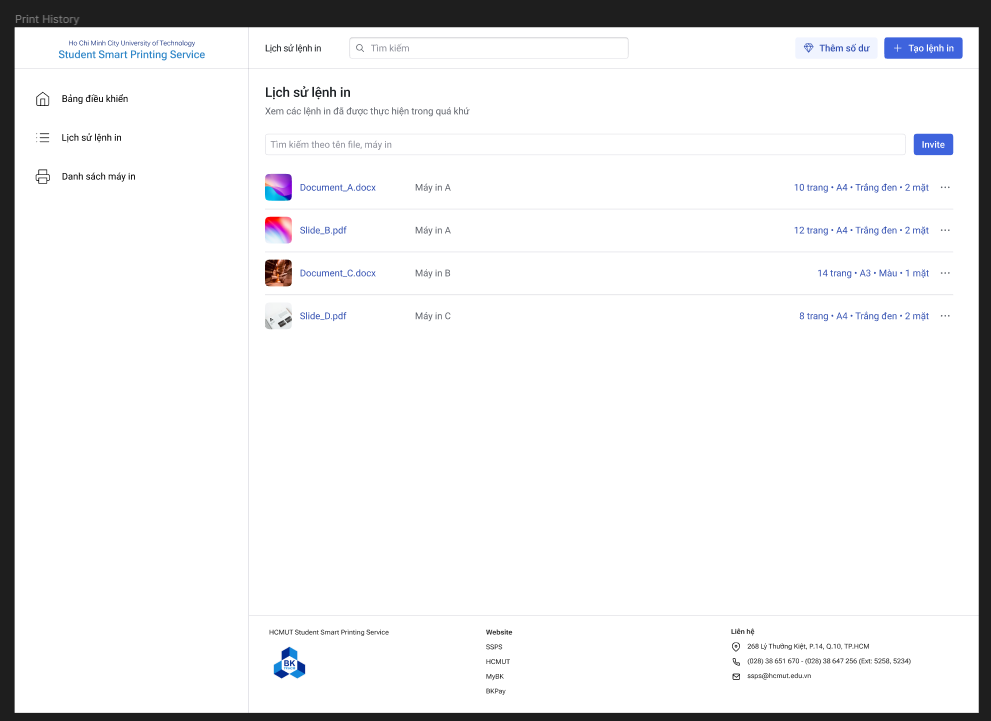
\includegraphics[max width=0.9\linewidth]{chapters/5. mvp-wireframe/5. Print History.png}
  \caption{Print History}%
\end{figure}

The Print History screen allows the user to view all their past print requests as well as the status of ongoing ones.

\begin{figure}[H]
  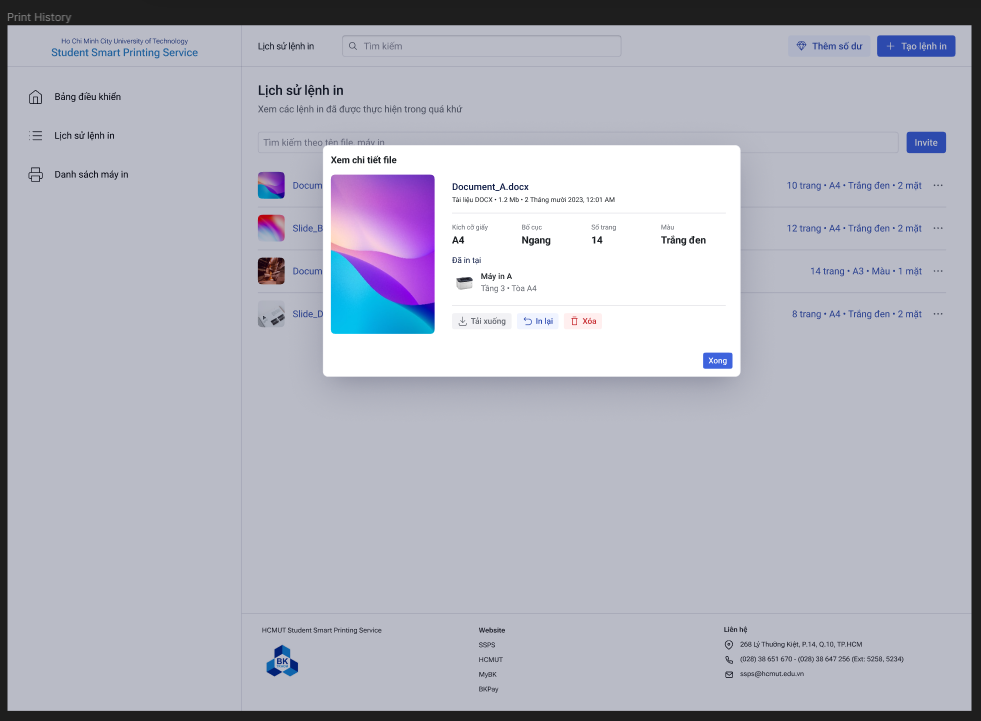
\includegraphics[max width=0.9\linewidth]{chapters/5. mvp-wireframe/6. Print History - Details.png}
  \caption{Print History - Detail view}%
\end{figure}

Clicking on one of the items from the list will open up the detail view, where the user can see all the details as well as performing actions like "Reprint the file", "Download the file", or "Delete the file".

\subsection{Printer List}

\begin{figure}[H]
  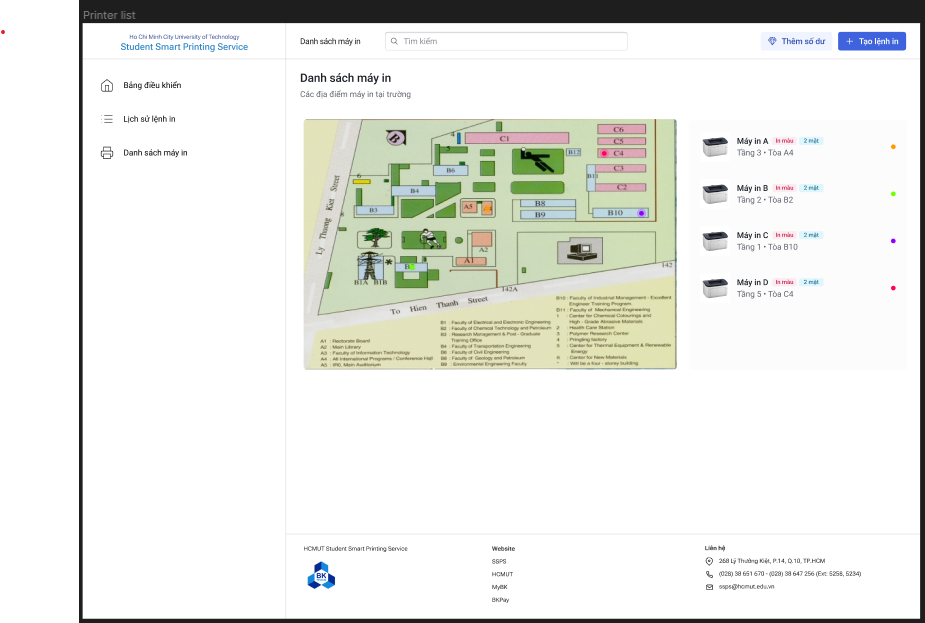
\includegraphics[max width=0.9\linewidth]{chapters/5. mvp-wireframe/7. Printer List.png}
  \caption{Printer List}%
\end{figure}

The Printer List view allows the user to view the list of all printers, their capabilities, and locations.

\begin{figure}[H]
  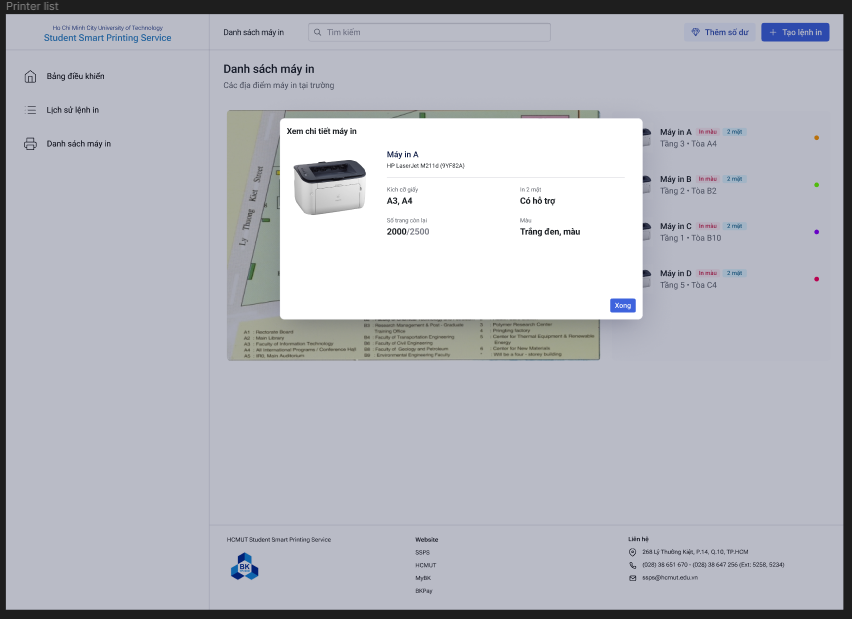
\includegraphics[max width=0.9\linewidth]{chapters/5. mvp-wireframe/8. Printer List - Details.png}
  \caption{Printer List - Detail view}%
\end{figure}

Clicking on one of the printer card will open a detailed view where the user can view all information about the printers.

\subsection{Admin Dashboard View}

The Dashboard admin view can be accessed using the same URL as the one in student view. Depending on the account role, different content is displayed.

\begin{figure}[H]
  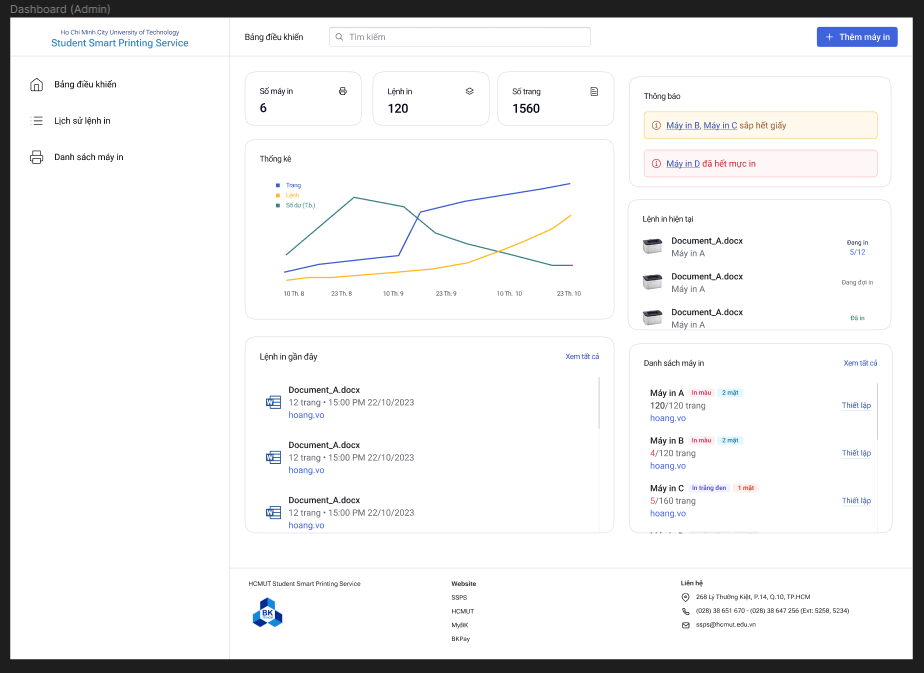
\includegraphics[max width=0.9\linewidth]{chapters/5. mvp-wireframe/9. Dashboard Admin.png}
  \caption{Admin Dashboard}%
\end{figure}

The dashboard admin view also gives the printing statistics but include data from all students.

\subsection{Add Printer}

\begin{figure}[H]
  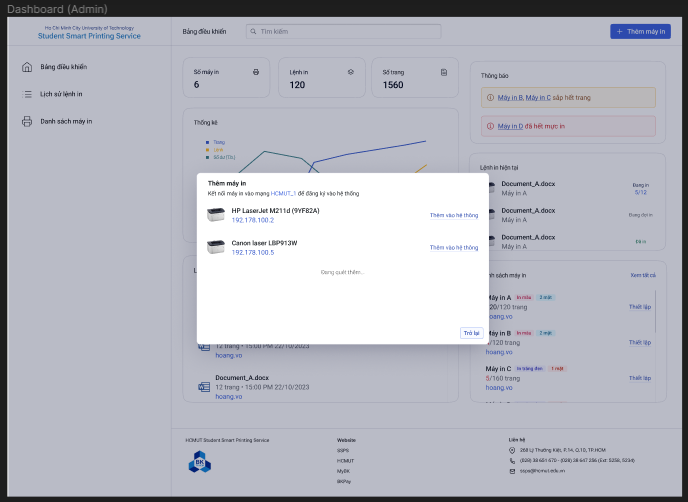
\includegraphics[max width=0.9\linewidth]{chapters/5. mvp-wireframe/10. Add Printer.png}
  \caption{Add Printer}%
\end{figure}

The admin can add new printers using the "Thêm máy in" button in the top right. After that the user can select a printer that can be discovered in the network or enter an IP Address.

\begin{figure}[H]
  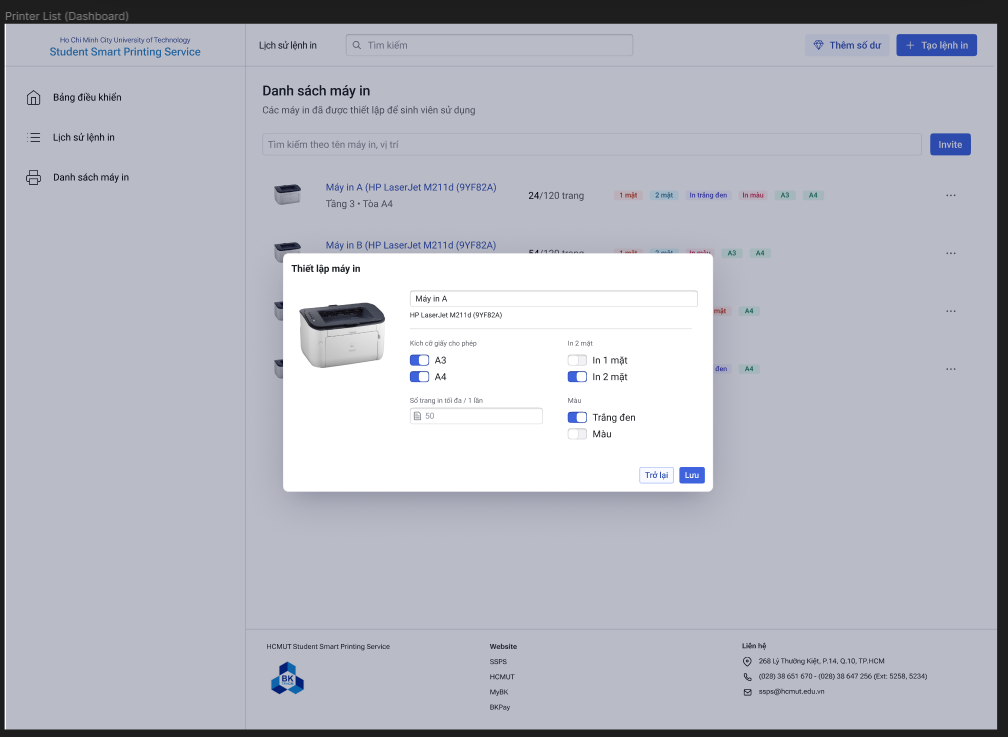
\includegraphics[max width=0.9\linewidth]{chapters/5. mvp-wireframe/12. Admin Printer Edit.png}
  \caption{Configure Printer}%
\end{figure}

The user can then configure the properties of the printers, which will determine the available options when users create a print request.

\subsection{Admin Printer List}

\begin{figure}[H]
  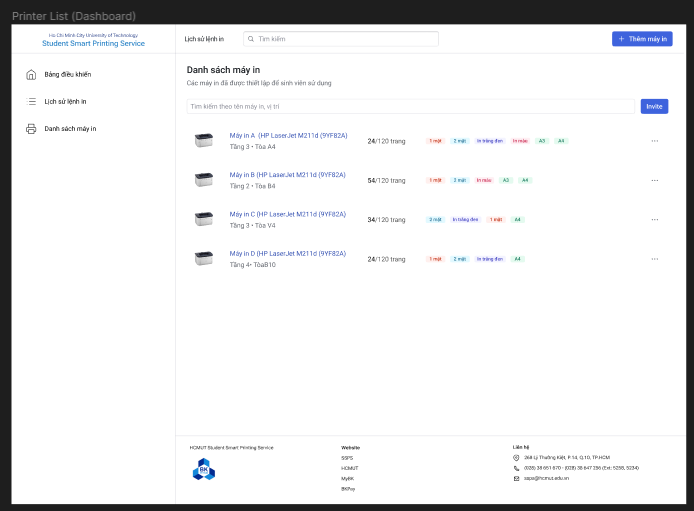
\includegraphics[max width=0.9\linewidth]{chapters/5. mvp-wireframe/11. Admin Printer List.png}
  \caption{Admin Printer List}%
\end{figure}

The admin printer list shows all printers as well as their configuration. Clicking on one of them will open up the printer configuration dialog as seen above.
\clearpage
\section{Layered Architecture}

\begin{figure}[H]
  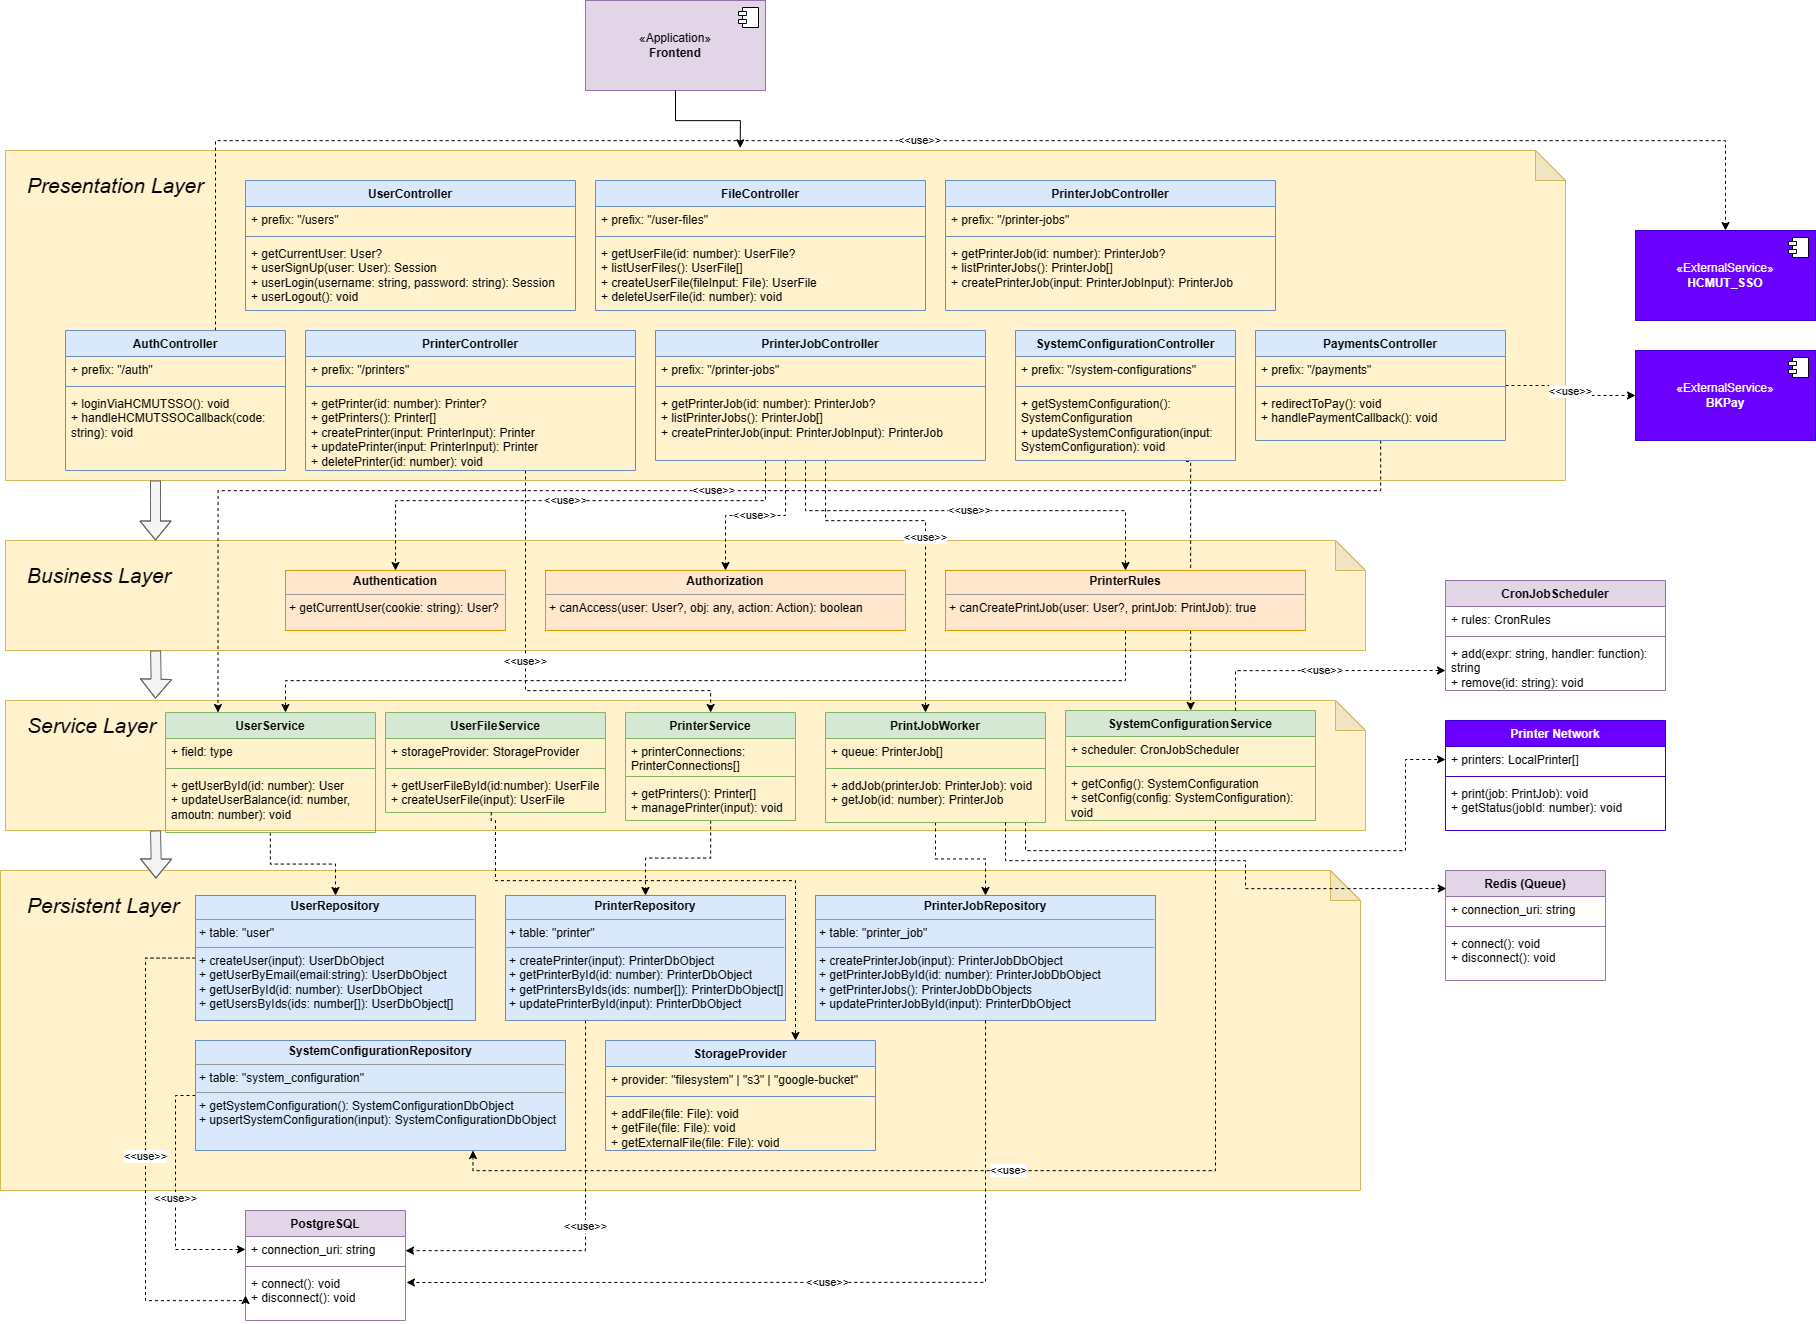
\includegraphics[max height=0.9\linewidth, angle=90,origin=c]{chapters/6. architecture-design/Architecture Diagram.drawio.png}
  \caption{Architecture Diagram}%
\end{figure}

The architecture diagram above demonstrates the layered architecture of our project. It is structured into a four-layer architecture, each serving distinct functions.

In our system architecture, data flow is designed to follow a unidirectional pattern, where each upper layer pulls data from the lower layer, but not vice versa. It somewhat resembles Onion Architecture\footnote{Pal, T. (2021, December 21). Understanding onion architecture. CodeGuru. https://www.codeguru.com/csharp/understanding-onion-architecture/}, whose design principle ensures a clear separation of concerns and enhances system maintainability and scalability. If we do not follow a unidirectional pattern, we can get into some issues like cyclic dependencies (imagine if a presentation component pulls data from a business logic component, but a business logic component in turns pulls data from the presentation component) and coupling.

\subsection{Presentation Layer}

\begin{figure}[H]
  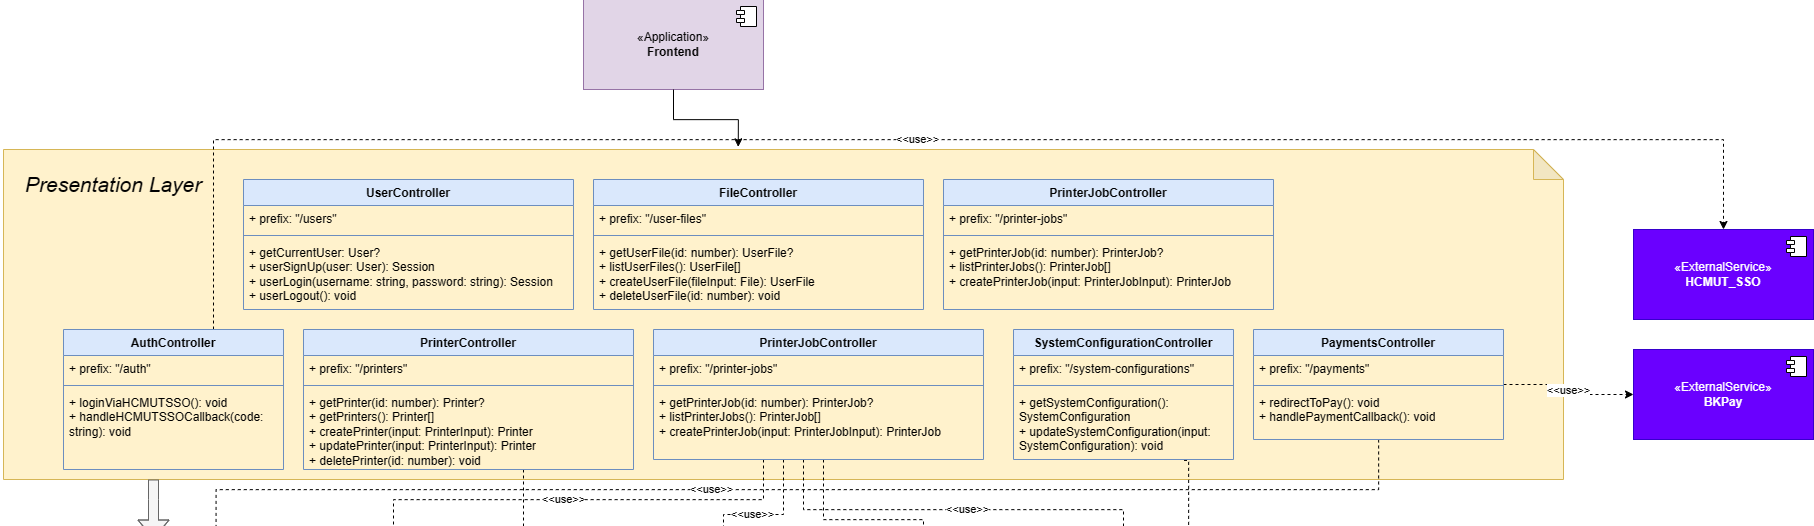
\includegraphics[max width=0.9\linewidth]{chapters/6. architecture-design/Layered Architecture/1. Presentation Layer.png}
  \caption{Presentation Layer}%
\end{figure}

This front-end layer features various controllers for user interaction, handling inputs and outputs for tasks like printing requests, document uploads, and navigating the app. Technically, the components’ interfaces are represented by REST endpoints that get called by the SSPS Mobile App and Web App. The Role of the Controller components are to process the web request by interacting with the service layer to complete the work that needs to be done.\footnote{G, A. (n.d.). Spring MVC Beginner’s Guide. O’Reilly Online Learning. https://www.oreilly.com/library/view/spring-mvc-beginners/9781783284870/ch03s03.html}\\

In our design, before interacting with the application/service layer, we also call onto components of Business Logic Layer to perform checks to ensure that the calling users should be able to call the respective application/service layer operation. For example, the user needs not only to be authenticated (validated using Business layer’s Authentication Service) but they must also be authorized to access the specified resource (validated using Business layer’s Authorization logic) - for example, user should be able to see only their uploaded documents and not anyone else and only admins should be able to make changes to the printer configurations. After receiving the result after calling the application/service layer, the controller layer forms the reasonable response to send back to the client, allowing them to display a UI accordingly to the user.\\

In some cases, the controllers of the presentation layer may also redirect users to some external resources to complete the operation of the lower layer. For example, to login, a controller may redirect the user to HCMUT\_SSO and handle the callback from that service to complete the authentication, or it may redirect the user to BKPAY to complete their page balance purchase. Last, the presentation layer also ensure that the input data is validated and formatted correctly before sending them of to the lower layers.

\subsection{Business Layer}

\begin{figure}[H]
  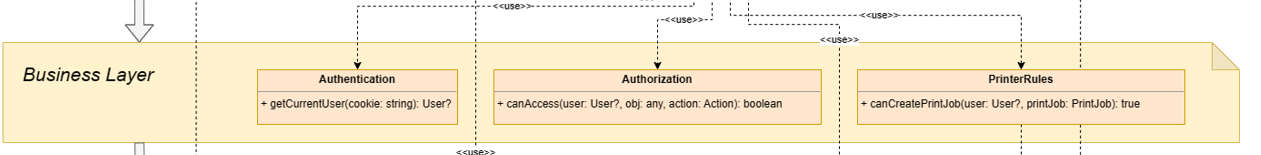
\includegraphics[max width=0.9\linewidth]{chapters/6. architecture-design/Layered Architecture/2. Business Layer.png}
  \caption{Business Layer}%
\end{figure}

Central to the system, this layer manages authentication, authorization, and adherence to printing rules, ensuring that user activities comply with system policies\footnote{Tesha, B. (2020b, March 12). Authentication/authorization is part of the business logic. Medium. https://medium.com/@benedict.tesha/authentication-authorization-is-part-of-the-business-logic-7d6c21627b8e}. The components in this layer are used by the presentation layer for it to make decisions before continuing onto the service layer.\\

To do its role, it must read into some components in the service layer. For example, to check authorization of the user to access a file, it must query the Document Service to determine the file owner to check against the current user. This abstraction is needed because, it should not know the implementation details of how a file is fetched (separation of concern) However, for some components, we may access the persistence layer directly to get the data. For example, for authentication, we query the token of the user from the App Session repository directly. This makes sense because everything authentication-related is handled by the business layer themselves and there is no need to add a corresponding service in the service layer. Separation of service layer and business logic layer is important because it allows the service layer to carry out its role independently. \\

Some components of the application (or internal processes) may call upon other components inside the service layer, in which case we should not need to perform any sort of authentication or authorization check, which is because in this case the caller of these operations is a system, which does not have the user involved. If we couple authentication inside the application, we will end up having to add exceptions to handle these internal use cases and would end up with an unmaintainable codebase. \\

Having a business layer before requests get routed to the service layer is obviously to ensure security and policy of the system and to make sense of business requirements like page balance.

\subsection{Service Layer}

\begin{figure}[H]
  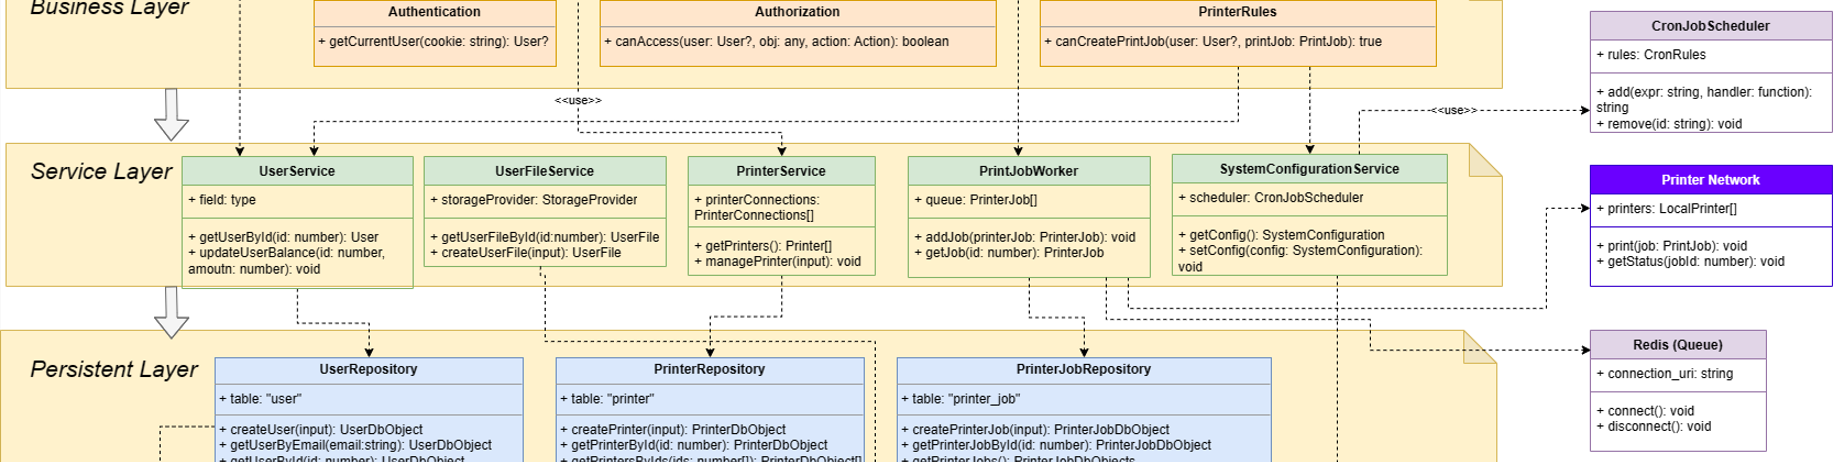
\includegraphics[max width=0.9\linewidth]{chapters/6. architecture-design/Layered Architecture/3. Service Layer.png}
  \caption{Service Layer}%
\end{figure}

Here, specialized services operate, including User Service for managing user information and balance, User File Service  for document and upload management, Payment Service for financial transactions, Printer Service for printer management and communication, Report Generator for creating reports, and Print Job Queue for organizing print jobs. The service layer / service layer centralizes logic to perform various tasks in the application. These logic is often organized into reusable modules for use by different aspects of the system, which allows the codebase to much more maintainable\footnote{Bedmutha, A. (2023, June 6). Why do we need Service layers? - Apoorv Bedmutha - Medium. Medium. https://medium.com/@bedmuthaapoorv/why-do-we-need-service-layers-ecf86ca5c739}.\\

In the case where other components of the system call another service, it is ideal because these other components must not know about implementation details of that service (how the data is fetched, written). This abstraction is helpful because along the way, the implementation detail of that service may change, but its public API remains the same, allowing other use cases to carry out as usual without having to make changes to accommodate.\\

Organizing logic into different services inside the application layer also makes it easier to manage and understand the dependencies between various services, which is important to ensure data requirement and flow are compatible.\footnote{ Parker, J. (2023, April 2). What is service layer in software architecture? - Architecture. Design Your World - Explore Architecture. https://www.architecturemaker.com/what-is-service-layer-in-software-architecture}. This organization is also particularly important in service-oriented architectures where services are shared and categorized into different layers.

\subsection{Persistent Layer}

\begin{figure}[H]
  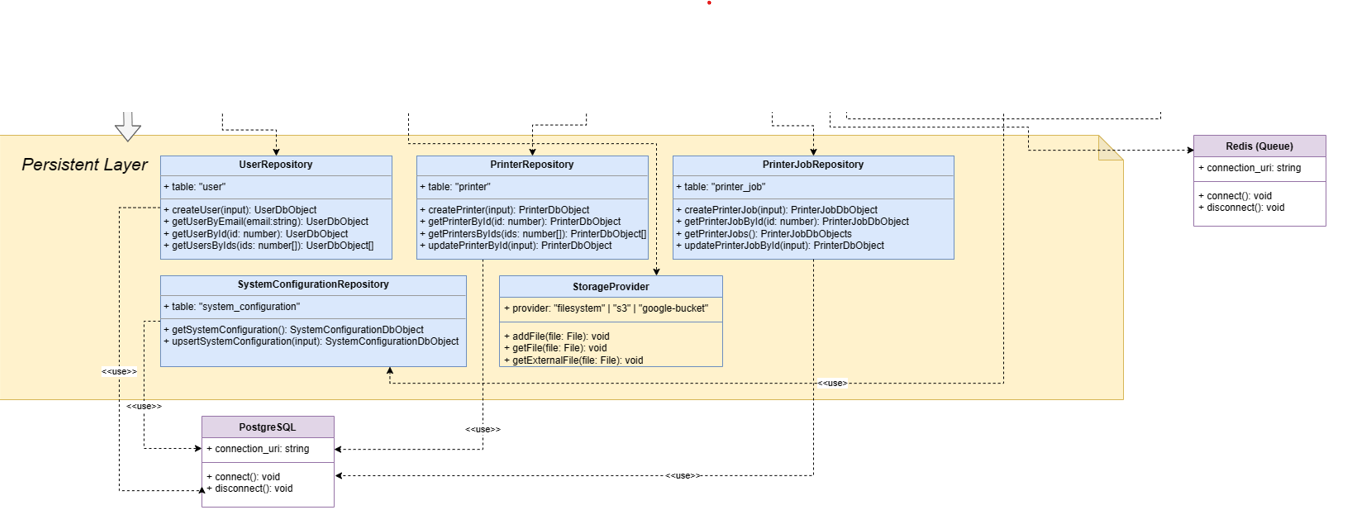
\includegraphics[max width=0.9\linewidth]{chapters/6. architecture-design/Layered Architecture/4. Persistent Layer.png}
  \caption{Persistent Layer}%
\end{figure}

Acting as an intermediary between the Service and underlying data provider, this layer consists of repositories for consistent and secure data transactions. They are abstractions to manage data storage and retrieval processes (operations to save, update, delete and query data). The abstraction of data source is helpful because it allows changes in the data storage without impacting the higher layer. For example, along the way, we might change from PostgreSQL to use a non-SQL database like MongoDB. This change does not require any changes from service code of the upper level because the repository class still maintains the same public APIs (eg. getUserById, getPrintingHistoryByUserId) as well as Data object (UserDbObject, PrinterDbObject). \\

In addition, this layer also ensures data integrity and security by enforcing validation rules and maintaining consistency across databases, which can be achieved by the abstraction of Database Object classes that perform validation upon initialization. Similarly, by removing the need for the upper layer to write database queries directly (given how different databases might have different syntax), we make the upper layer’s code more maintainable and more resilient against changes in the infrastructure (database system component for specific)\footnote{Jamesmontemagno. (2023, February 21). Designing the infrastructure persistence layer - .NET. Microsoft Learn. https://learn.microsoft.com/en-us/dotnet/architecture/microservices/microservice-ddd-cqrs-patterns/infrastructure-persistence-layer-design
}.\\

\section{Component diagrams}
\subsection{Printing Service}
\begin{figure}[H]
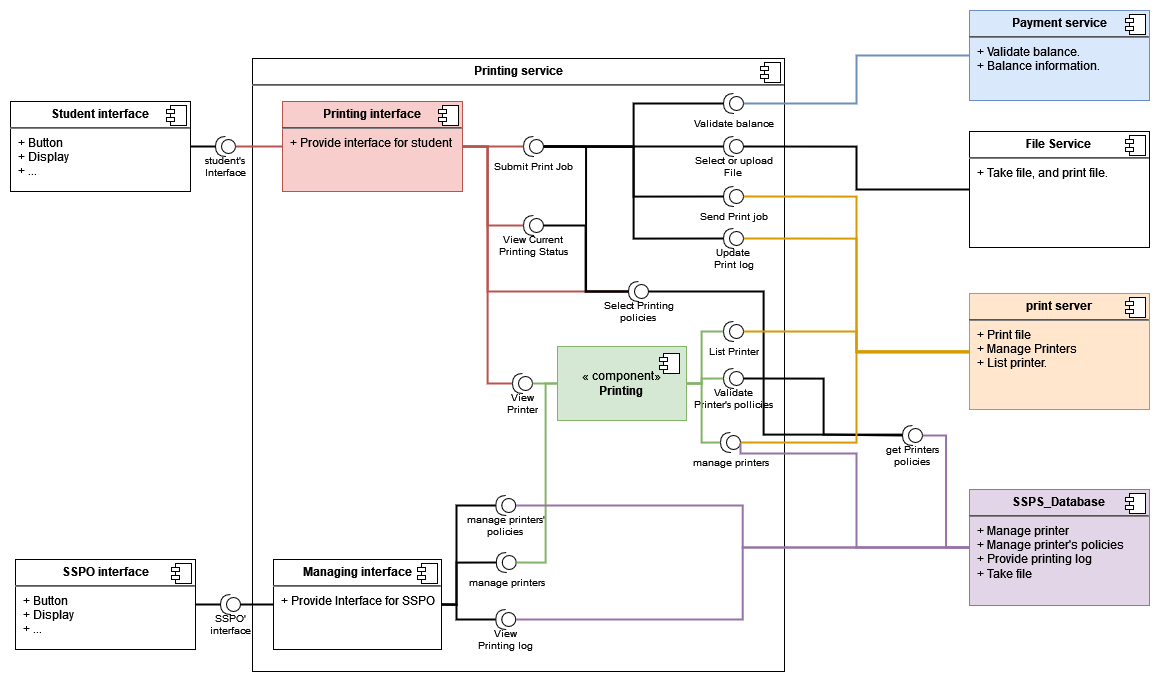
\includegraphics[max width = 0.9\linewidth,origin = c]{chapters/6. architecture-design/Component Diagram/printing.png}
  \caption{Printing service}%
  \end{figure}

This diagram represents the architecture of the printing service system, which is composed of five main components, each with distinct functionalities: 
\begin {enumerate}
    \item \textbf{Managing and Printing Interfaces:} These interfaces are crucial for interaction, designed to handle and efficiently respond to inputs from both students and the Student Services and Programs Office (SSPO). They enable a user-friendly experience for managing print jobs and provide real-time feedback.
    \item \textbf{Printer Manager:} A vital component that facilitates communication with the print server. It's responsible for the operational aspects of printing, including queue management, printer status monitoring, and error handling. This manager ensures that the printing process is smooth and efficient.
    
\end{enumerate}
    Beside main components in the service, the printing service also provide some interfaces from other components and services. This also show the relationships between service are important. \\
\subsection{Payment service}
\begin{figure}[H]
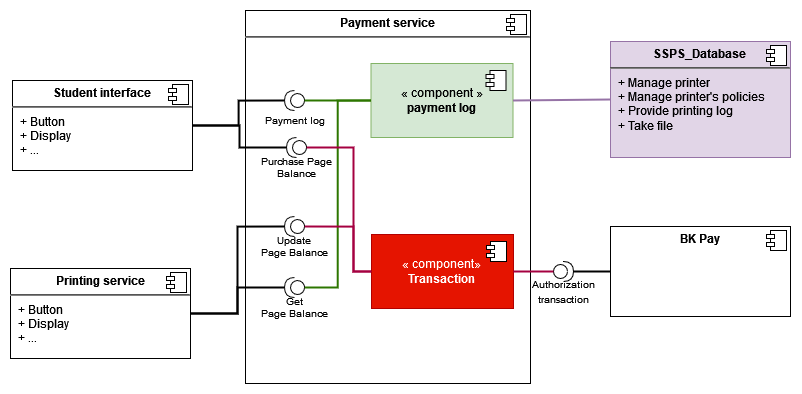
\includegraphics[max width = 0.9\linewidth,origin = c]{chapters/6. architecture-design/Component Diagram/payment.png}
  \caption{Payment service}%
  \end{figure}
Expanding on the Payment Service, it includes two main components with specific roles:
\begin{enumerate}
    \item \textbf{Payment Log:} This component is dedicated to recording and maintaining a comprehensive log of all payment transactions. It is essential for tracking payment histories, verifying transactions, and providing users and administrators with detailed financial reports.
    \item \textbf{Transaction:} It focuses on managing the actual transaction processes. This includes handling various payment methods, securing transaction data, and ensuring the efficient processing of user payments. It is designed to be robust and secure, capable of handling high volumes of transactions with accuracy.
\end{enumerate}
This service also extends its functionalities to the printing service, offering integration methods that allow for seamless financial transactions within the printing system.



\subsection{User Authentication service and reporting service}
\begin{figure}[H]
    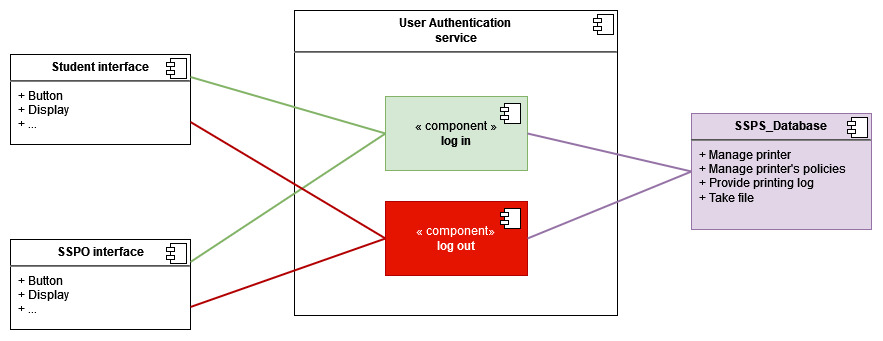
\includegraphics[max width = 0.9\linewidth,origin = c]{chapters/6. architecture-design/Component Diagram/Login.jpg}
    \caption{User Authentication service}%
\end{figure}

\begin{figure}[H]
    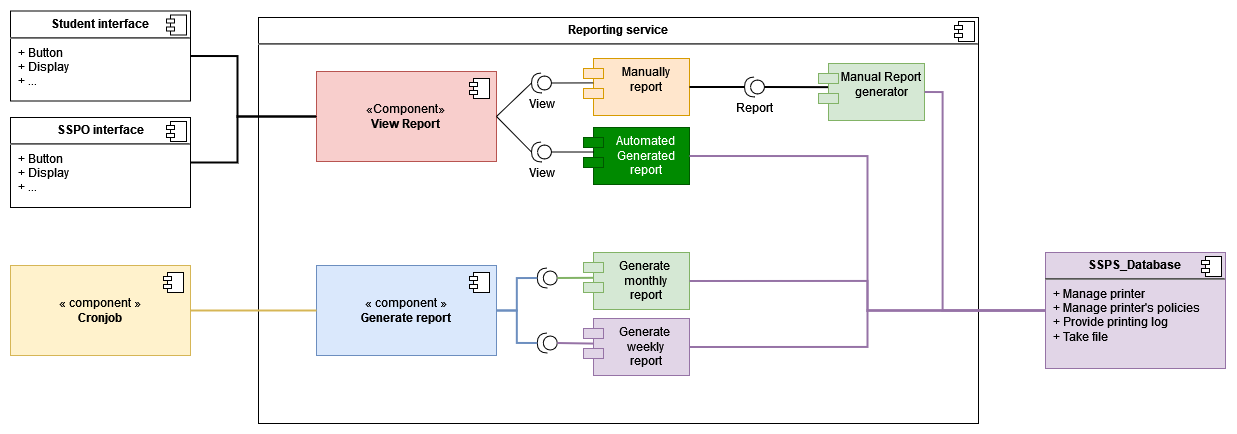
\includegraphics[max width = 0.9\linewidth,origin = c]{chapters/6. architecture-design/Component Diagram/report.png}
    \caption{Reporting service}%
\end{figure}
Lastly, the system encompasses additional modules, such as:
\begin{enumerate}
    \item \textbf{User Authentication Service:} This module is responsible for securing the system by managing user logins and logouts. It employs robust security protocols to ensure user identity verification, access control, and data protection.
    \item \textbf{Reporting Service:} This service is designed to compile and provide comprehensive reports on various aspects, such as usage statistics, operational performance, and financial summaries. It can generate weekly or monthly reports, offering valuable insights for management and decision-making processes.
\end{enumerate}
These services not only enhance the overall system functionality but also ensure operational integrity and user satisfaction.
\clearpage

\section{Implementation – Sprint 1}

\subsection{Setting up an online repository (github, bitbucket, etc) for version control.}

We have set up a repository at: \href{https://github.com/hoangvvo/CO3001-SmartStudentPrintingService}{Git hub repository}
\subsection{Adding documents, materials and folders for Requirement, System modelling and Architectural design.}
Documents, materials, and folders for requirement, system modeling and architecture design have been added to the `docs` folder.
\begin{figure}[H]
    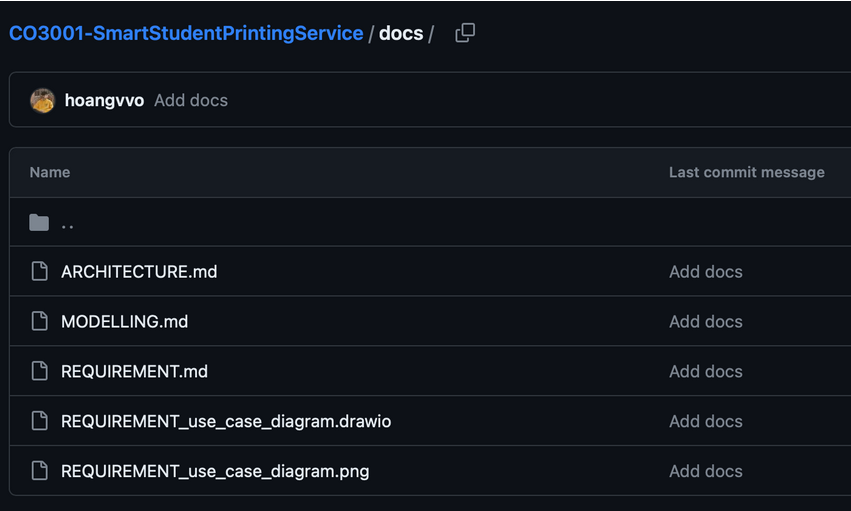
\includegraphics[max width = 0.9\linewidth,origin = c]{chapters/7. Implementation – Sprint 1/document,vv.png}
    \caption{Repository}%
\end{figure}

\subsection{Conducted a usability test with the user interface you developed in MVP 1.}
The following questions are used in the questionnaire to conduct the usability test. The test is performed online using Google Form.\\
The form can be found here: \href{https://forms.gle/c92x9Q3QJvYeMsRH6}{Google Form}
\subsubsection{Questions}
\textit{Basic questions:}
\begin{enumerate}
    \item Bạn đang học tập/công tác ở đâu?
    \item Bạn đang là sinh viên năm mấy?
    \item Bạn là sinh viên khoa…
\end{enumerate}
\indent \indent The reason for the basic questions is to understand the demography of the surveyees.\\
\indent \textit{Feedback questions:}\\
\indent \indent We are testing against the following features: Dashboard, Upload function, Print History, and Printer List.\\
\indent \indent For each page, we ask a series of grid multiple choice questions:
\begin{enumerate}
    \item Dễ sử dụng
    \item Thiết kế và thẩm mỹ
    \item Đáp ứng đầy đủ yêu cầu
\end{enumerate}
\indent \indent Each question can be answered from 1 (Strongly disagreed) to 5 (Strongly agreed).
\subsubsection{Responses}
The responses are collected in this Google Sheet: \href{https://docs.google.com/spreadsheets/d/19ywJ2WqR-1UwOe_dwIv6s4Ub5834-oyfKyqbfBqh974/edit#gid=1365939538}{Google Sheet}\\
\indent Here's a breakdown of the average ratings for each component of the application, considering the three aspects: Ease of Use, Design and Aesthetics, and Fulfillment of Requirements.\\
\indent Dashboard
\begin{itemize}[label =$\bullet$]
    \item \textbf{Ease of Use:} Average rating of about 3.02, indicating a moderate level of user-friendliness.
    \item \textbf{Design and Aesthetics:} Slightly lower rating of approximately 2.93, suggesting that the design might need improvements for better appeal.
    \item \textbf{Fulfillment of Requirements:} Average rating of around 3.07, showing that it moderately meets user needs.
\end{itemize}
\indent \indent Upload function
\begin{itemize}[label =$\bullet$]
    \item \textbf{Ease of Use:} Slightly higher average rating of approximately 3.09, indicating it's relatively user-friendly.
    \item \textbf{Design and Aesthetics:} Similar rating of about 3.07, suggesting an average design quality.
    \item \textbf{Fulfillment of Requirements:} A rating of around 3.12, which is slightly better, indicating it meets user needs well.
\end{itemize}
\indent \indent Print history
\begin{itemize}[label =$\bullet$]
    \item \textbf{Ease of Use:} A higher rating of around 3.16, suggesting good user-friendliness.
    \item \textbf{Design and Aesthetics:} Also higher, at about 3.12, indicating a more favorable design.
    \item \textbf{Fulfillment of Requirements:} Similar rating of approximately 3.09, showing it meets user needs adequately.
\end{itemize}
\indent \indent Printer List
\begin{itemize}[label =$\bullet$]
    \item \textbf{Ease of Use:} Average rating of about 3.07, indicating moderate ease of use.
    \item \textbf{Design and Aesthetics:} A bit lower at around 2.98, suggesting the design could be improved.
    \item \textbf{Fulfillment of Requirements:} An average rating of 3.0, indicating it meets user needs to a moderate extent.
\end{itemize}
\subsubsection{Conclusion}
In summary, the Print History component seems to be performing the best overall, with relatively higher ratings in all aspects. The Dashboard and Printer List components have lower ratings in design, which could be an area for improvement. The Upload function scores well in fulfilling user requirements, but its ease of use and design are average.


\clearpage

\section{Final Product}

Below is the final product of our project. 

\subsection{Resources}

For online demo, please check out the following link\\
\indent\indent \href{https://co-3001-smart-student-printing-service.vercel.app}{https://co-3001-smart-student-printing-service.vercel.app}
\\
\indent For demo video, please check out the following\\
\indent \indent \href{https://drive.google.com/drive/u/1/folders/1nSVqsj9_NubFQLUs2wFIGpq8M5zzPma2}{Google Drive - Presentation folder}
\\
\indent The presentation file can be accessed online via Canva:
\\
\indent \indent \href{https://www.canva.com/design/DAF2IG6wHOs/ovgEZU43pdSsiCqPl_B5uw/view}{Canva - Group 14-CC02 Smart Student Printing Service}
\\
\indent A PDF version can be found here:
\\
\indent \indent \href{https://drive.google.com/file/d/1c7-psaLMC4-su2_llzabOld_COfxqFA7/view?usp=sharing}{Google Drive - Group 14-CC02 Smart Student Printing Service}
\\

\subsection{Screenshots}

\subsubsection{Dashboard}

\begin{figure}[H]
    \centering
    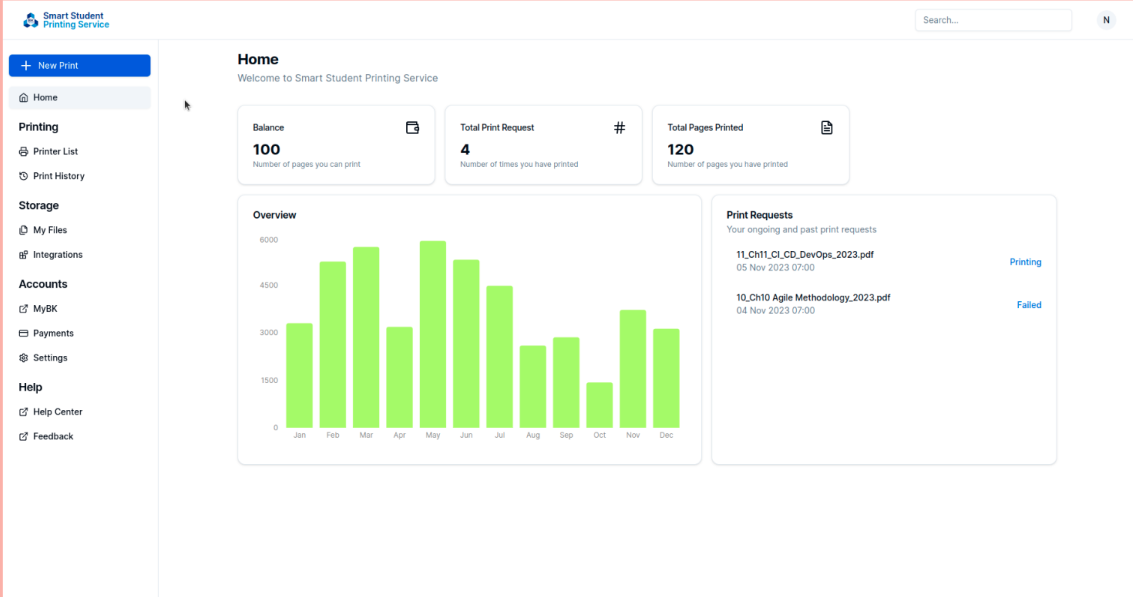
\includegraphics[max width = 0.9\linewidth,origin = c]{chapters/8. Implementation - Sprint 2/1. Dashboard.png}
    \caption{Dashboard}%
\end{figure}

\subsubsection{Create print job}

\begin{figure}[H]
    \centering
    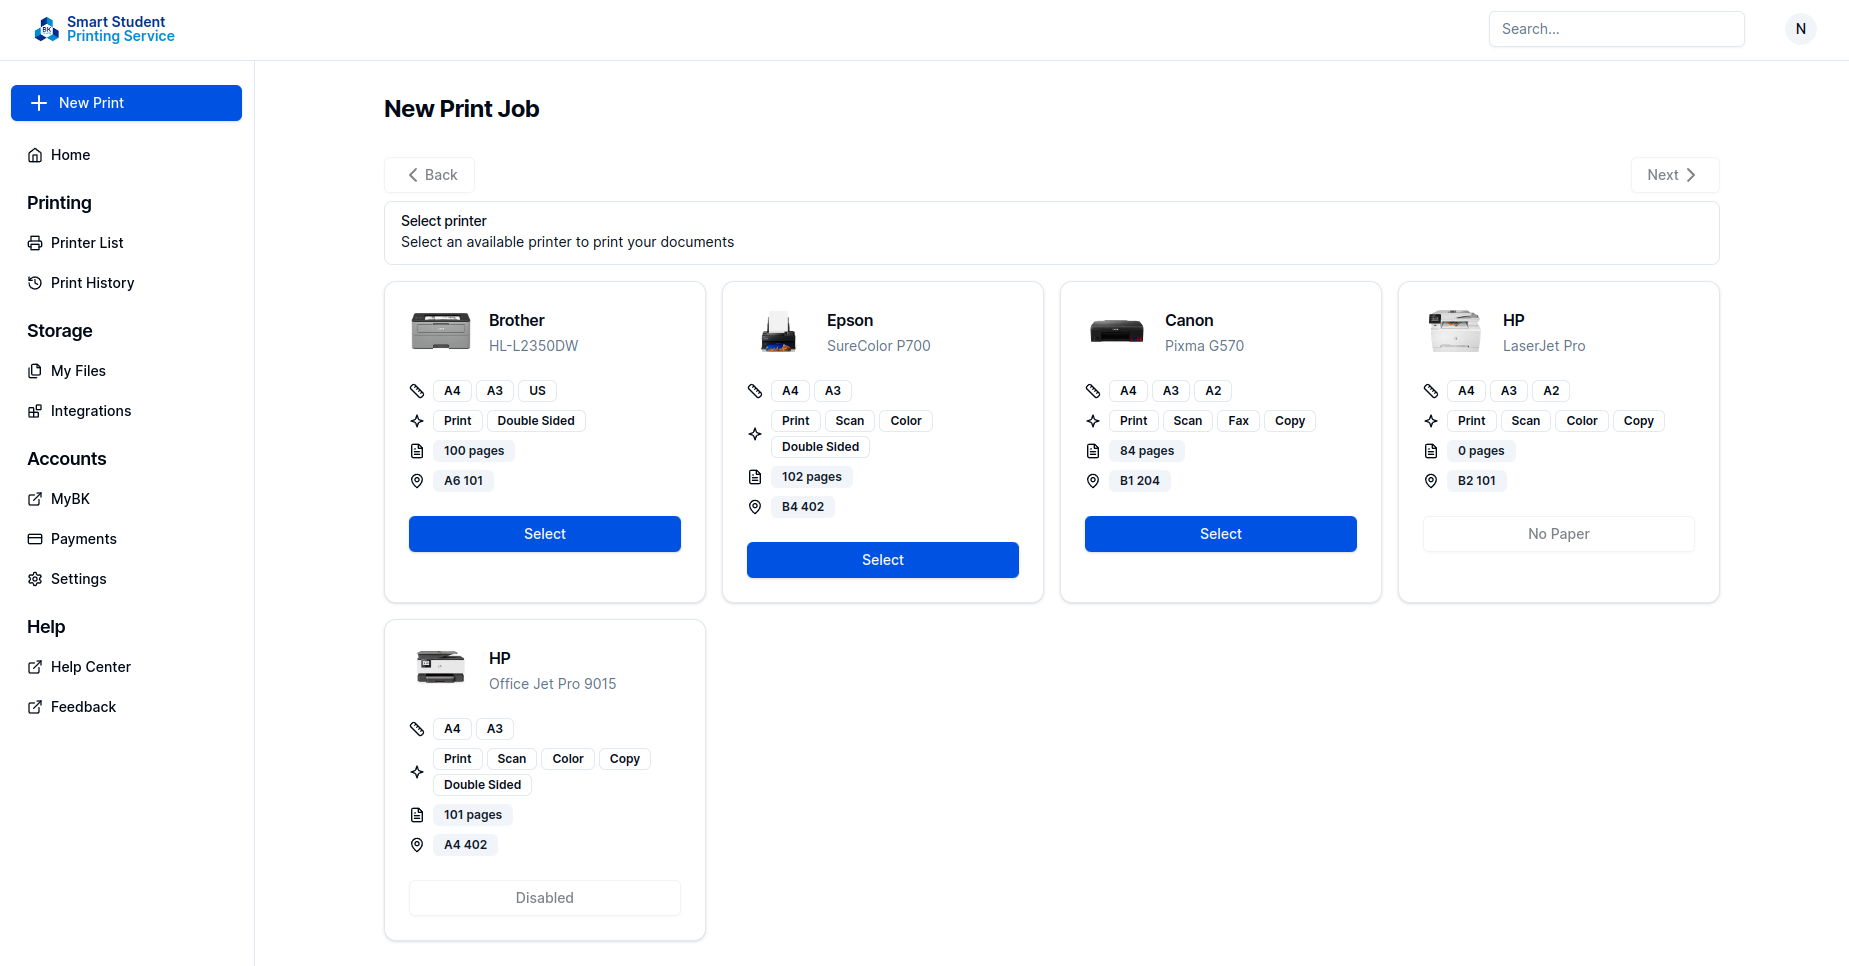
\includegraphics[max width = 0.9\linewidth,origin = c]{chapters/8. Implementation - Sprint 2/2. Create print job.png}
    \caption{Create Print Job - Select Printer}%
\end{figure}


\begin{figure}[H]
    \centering
    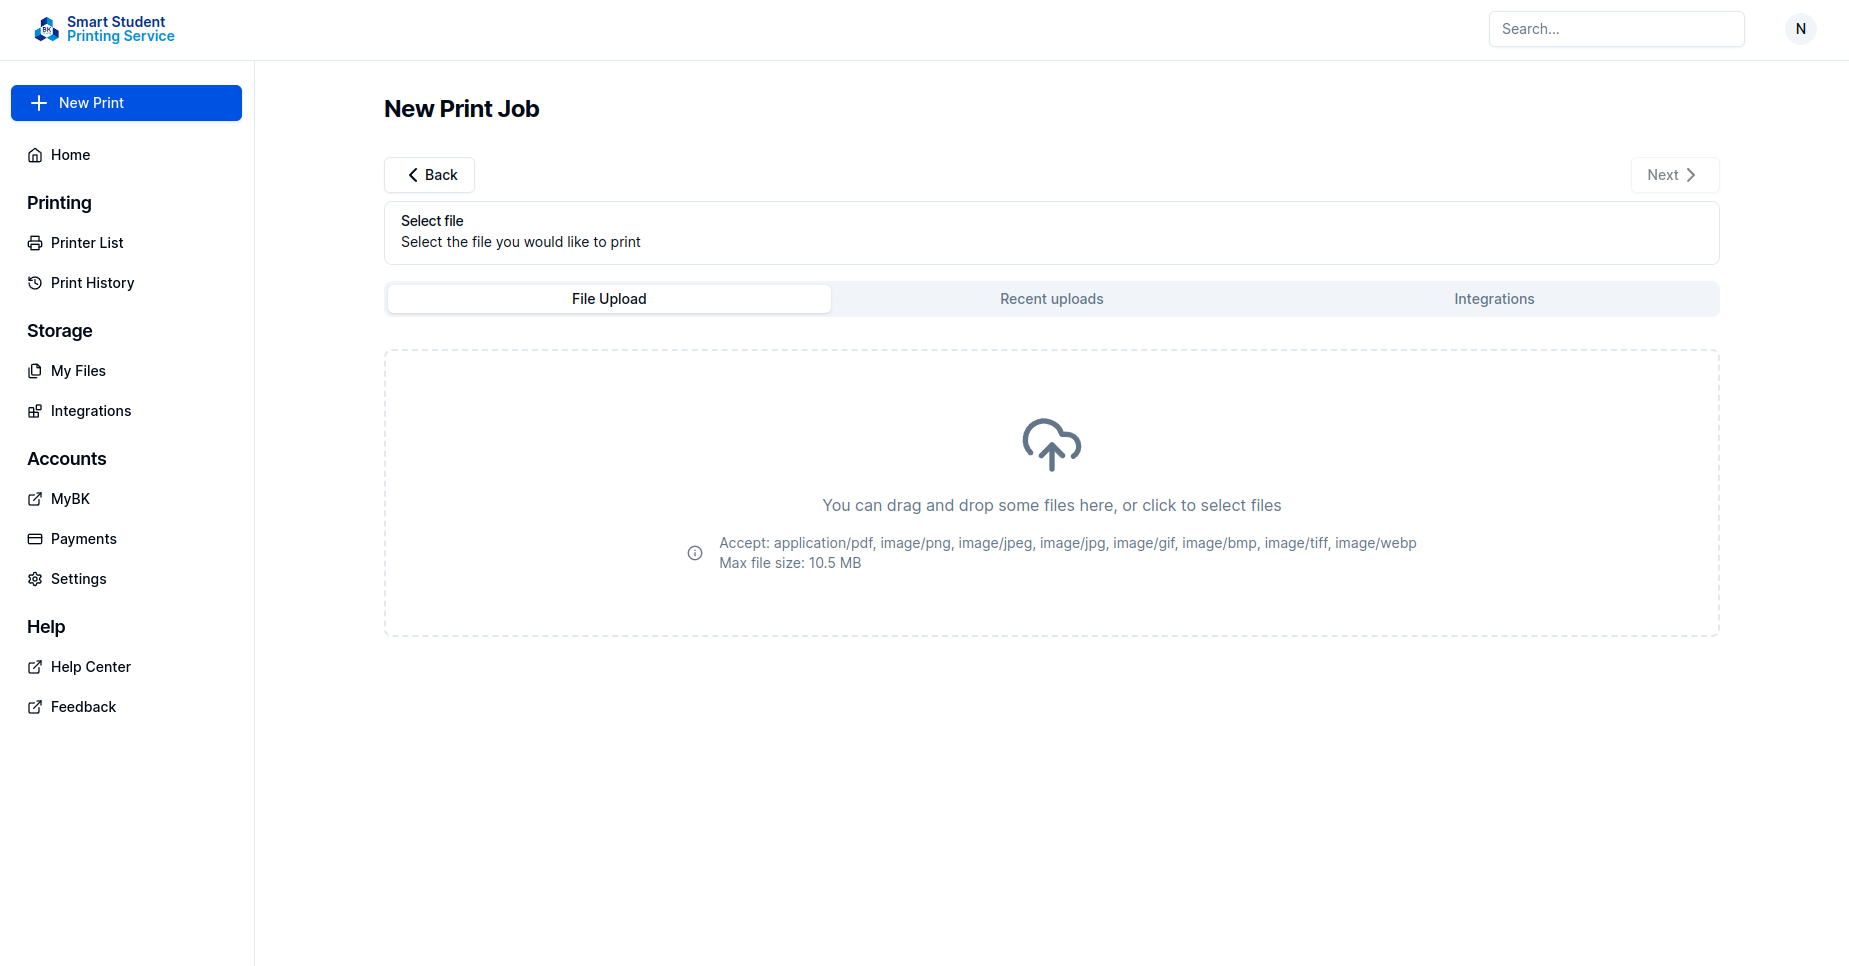
\includegraphics[max width = 0.9\linewidth,origin = c]{chapters/8. Implementation - Sprint 2/3. Create print job - select file - upload.png}
    \caption{Create Print Job - Select File - Upload}%
\end{figure}
\begin{figure}[H]
    \centering
    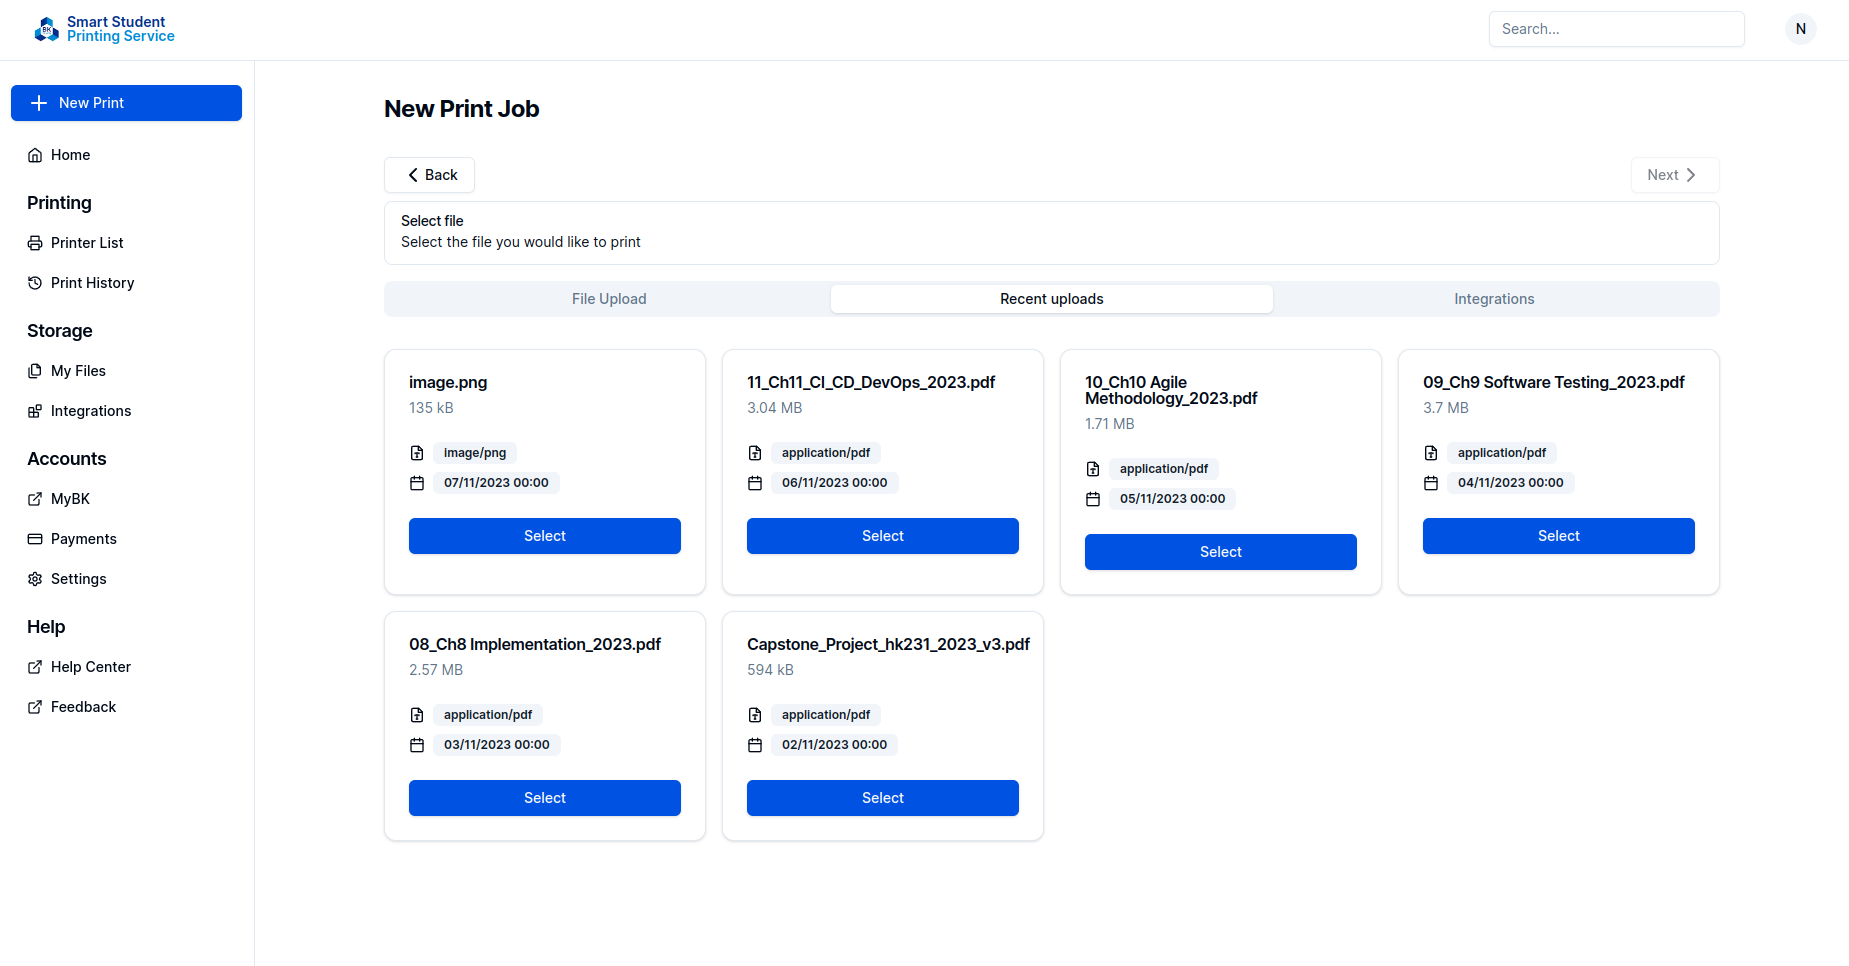
\includegraphics[max width = 0.9\linewidth,origin = c]{chapters/8. Implementation - Sprint 2/4. Create print job - select file - recent.png}
    \caption{Create Print Job - Select File - From recent uploads}%
\end{figure}
\begin{figure}[H]
    \centering
    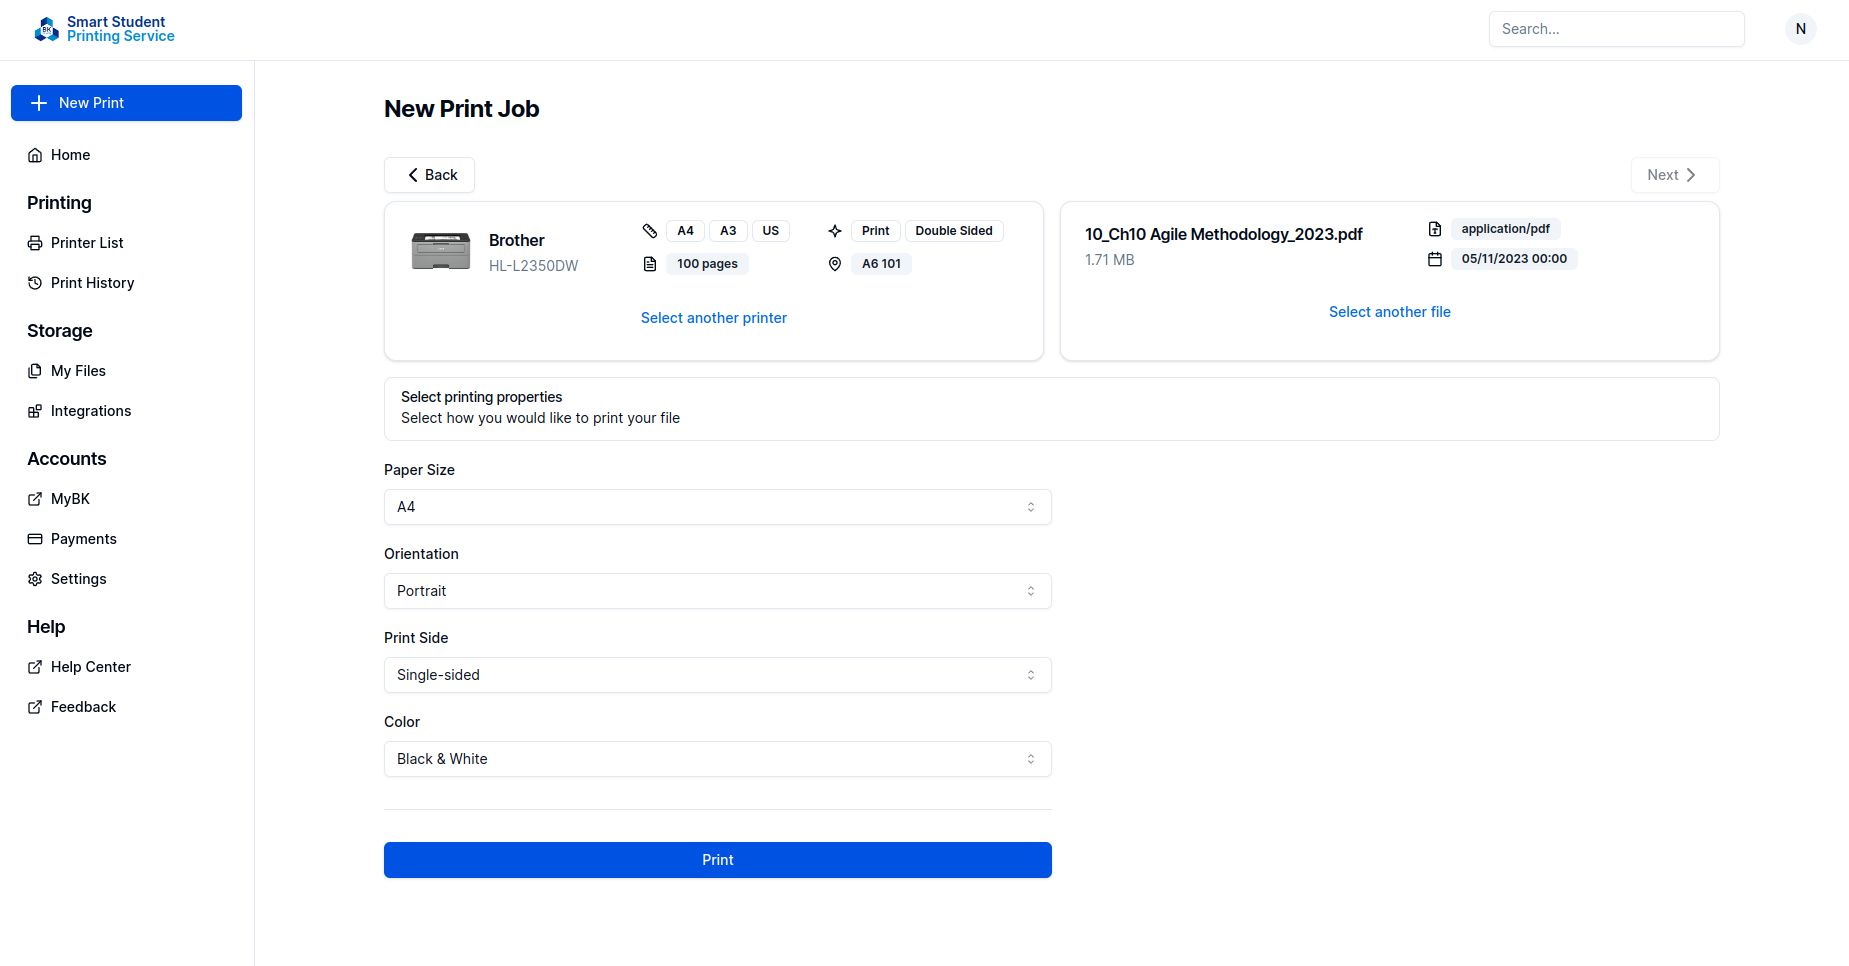
\includegraphics[max width = 0.9\linewidth,origin = c]{chapters/8. Implementation - Sprint 2/5. Create print job - select properties.png}
    \caption{Create Print Job - Select Printing Properies}%
\end{figure}

\subsubsection{Printer List}

\begin{figure}[H]
    \centering
    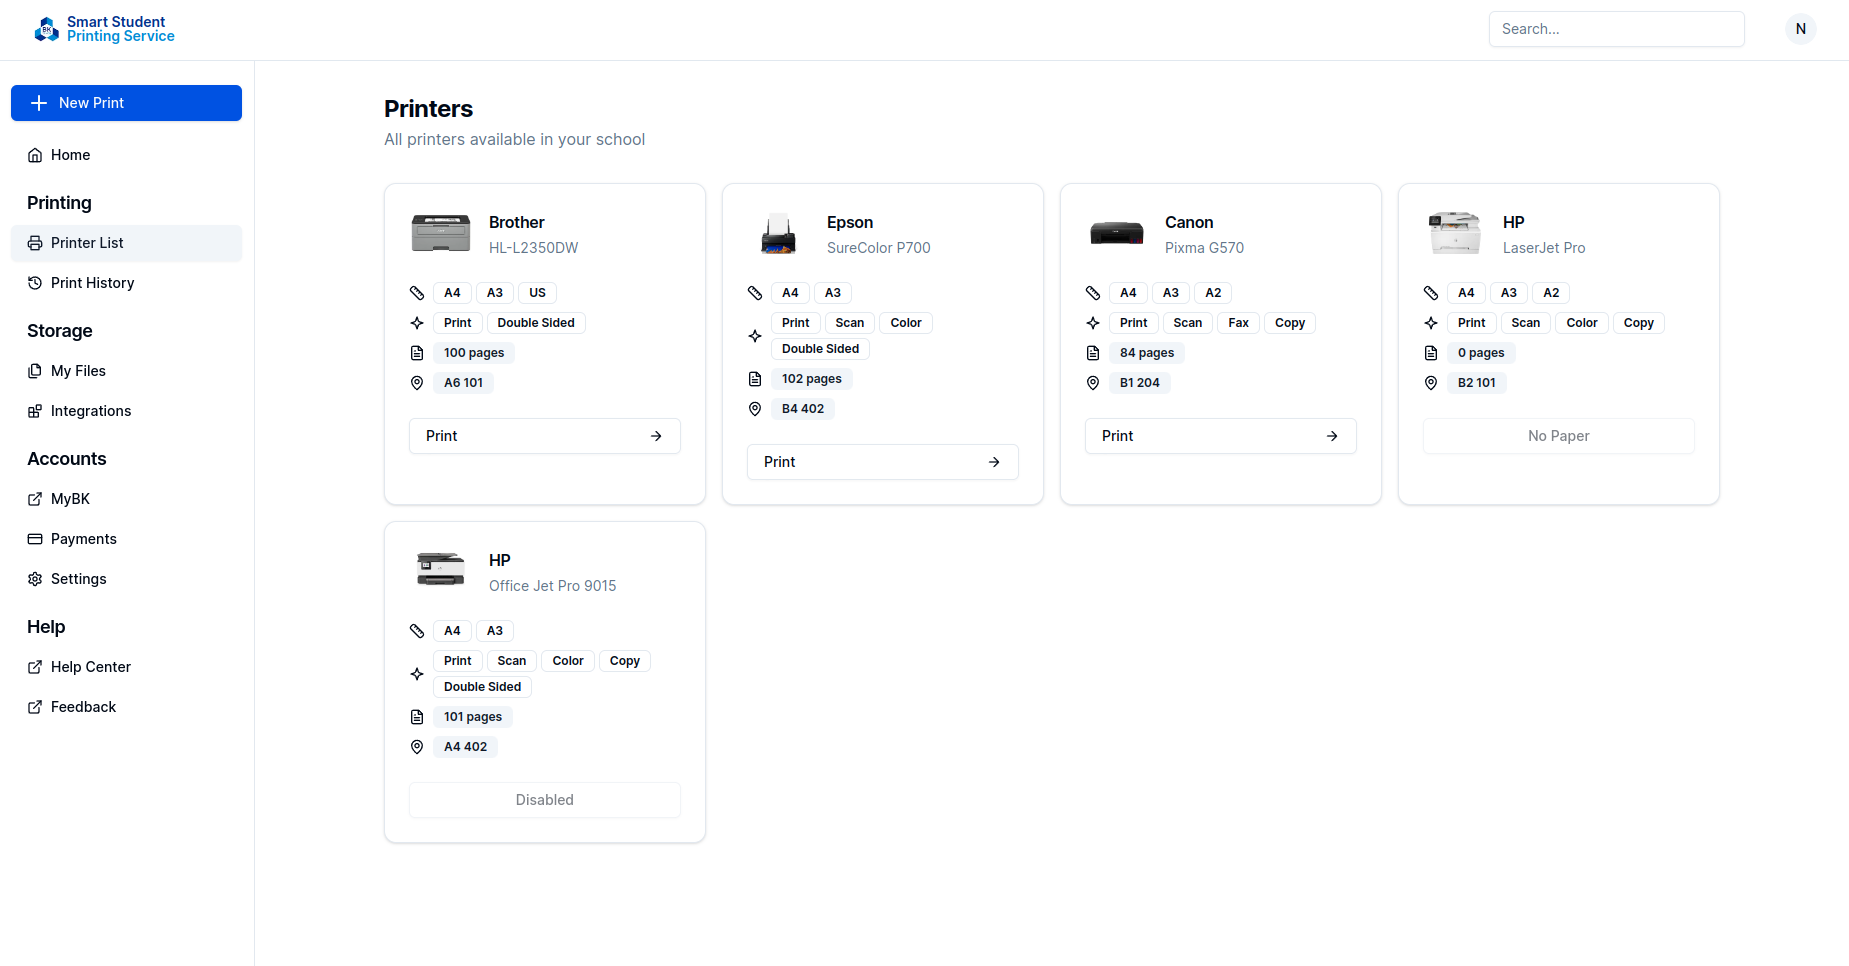
\includegraphics[max width = 0.9\linewidth,origin = c]{chapters/8. Implementation - Sprint 2/6. Printer list.png}
    \caption{Printer List}%
\end{figure}

\subsubsection{Printing History}

\begin{figure}[H]
    \centering
    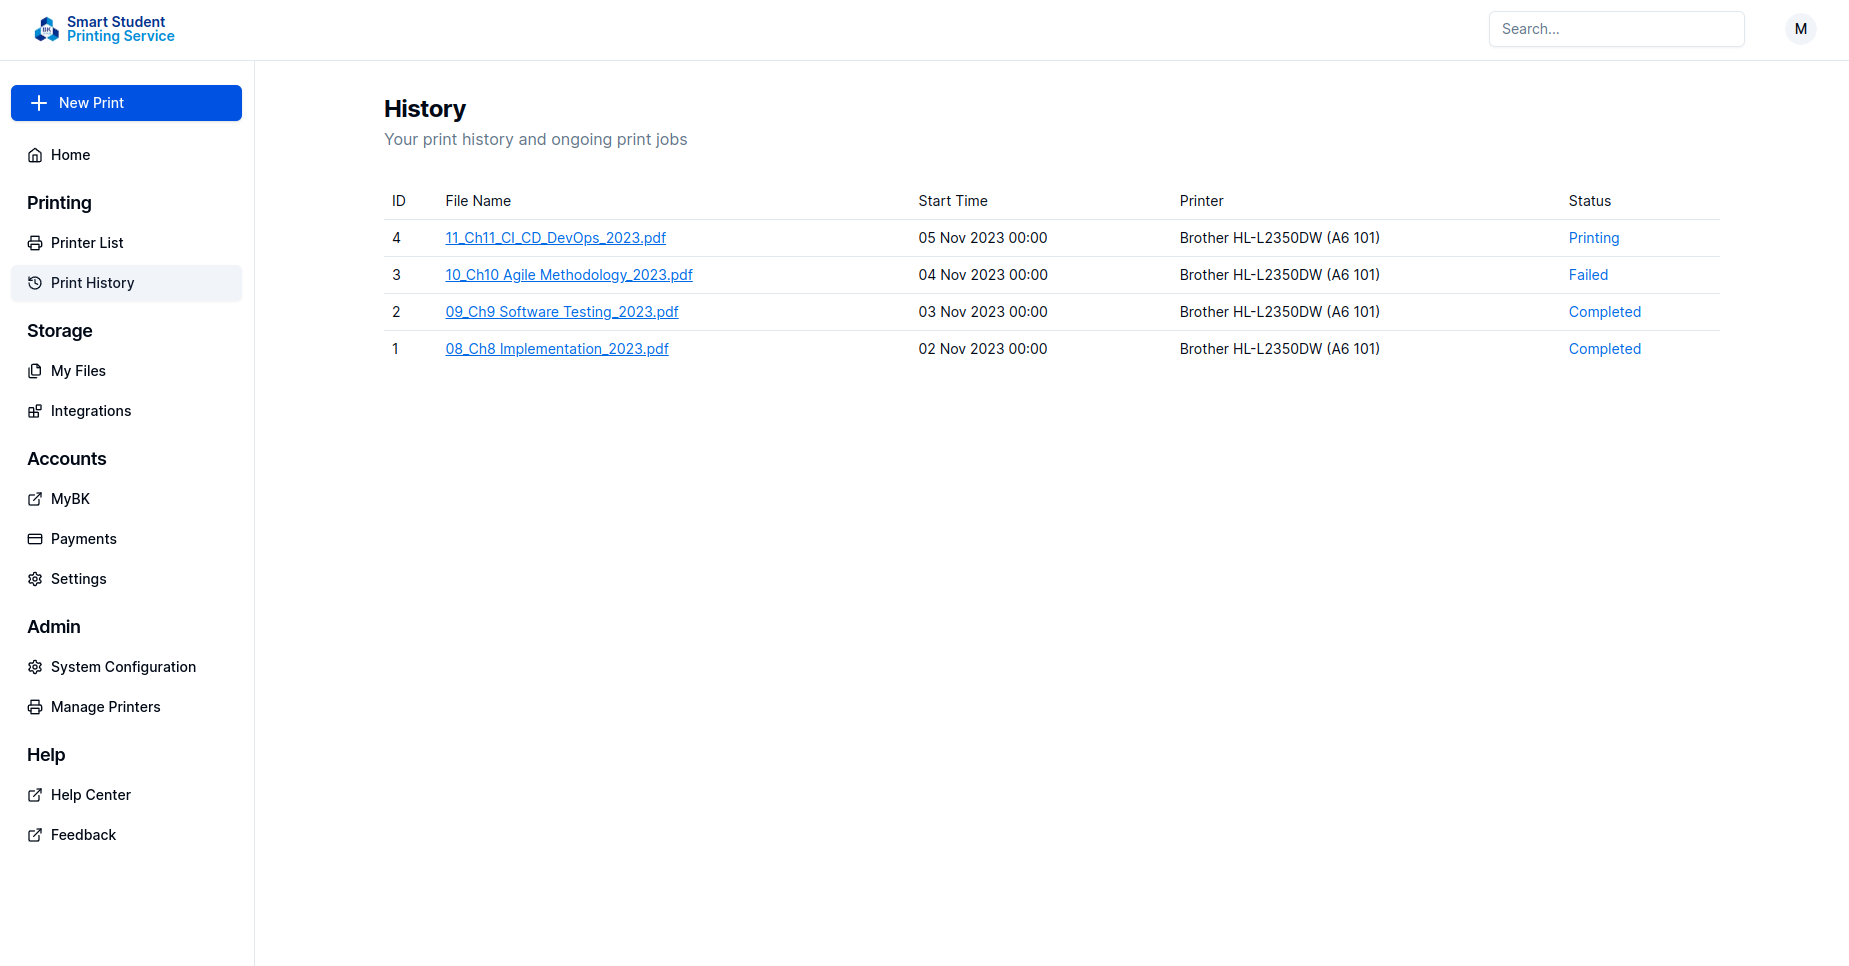
\includegraphics[max width = 0.9\linewidth,origin = c]{chapters/8. Implementation - Sprint 2/7. print history.png}
    \caption{Printing History}%
\end{figure}

\subsubsection{Files Management}

\begin{figure}[H]
    \centering
    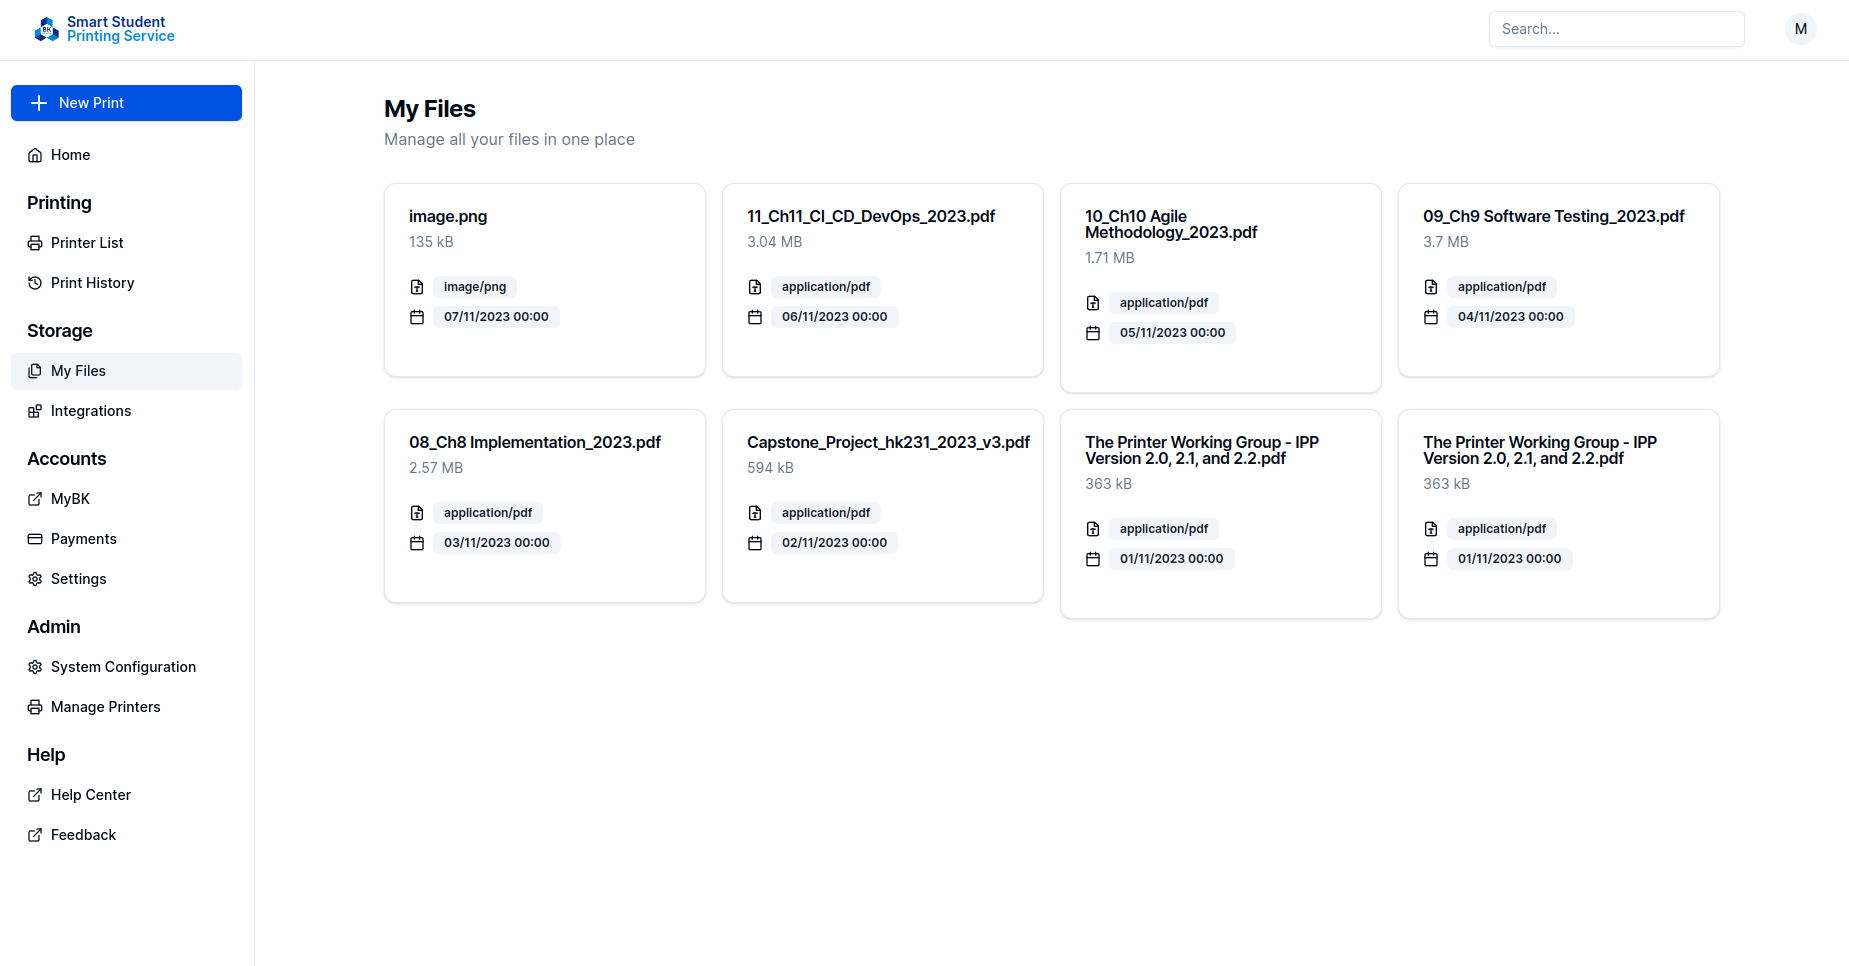
\includegraphics[max width = 0.9\linewidth,origin = c]{chapters/8. Implementation - Sprint 2/8. my files.png}
    \caption{My Files}%
\end{figure}
\begin{figure}[H]
    \centering
    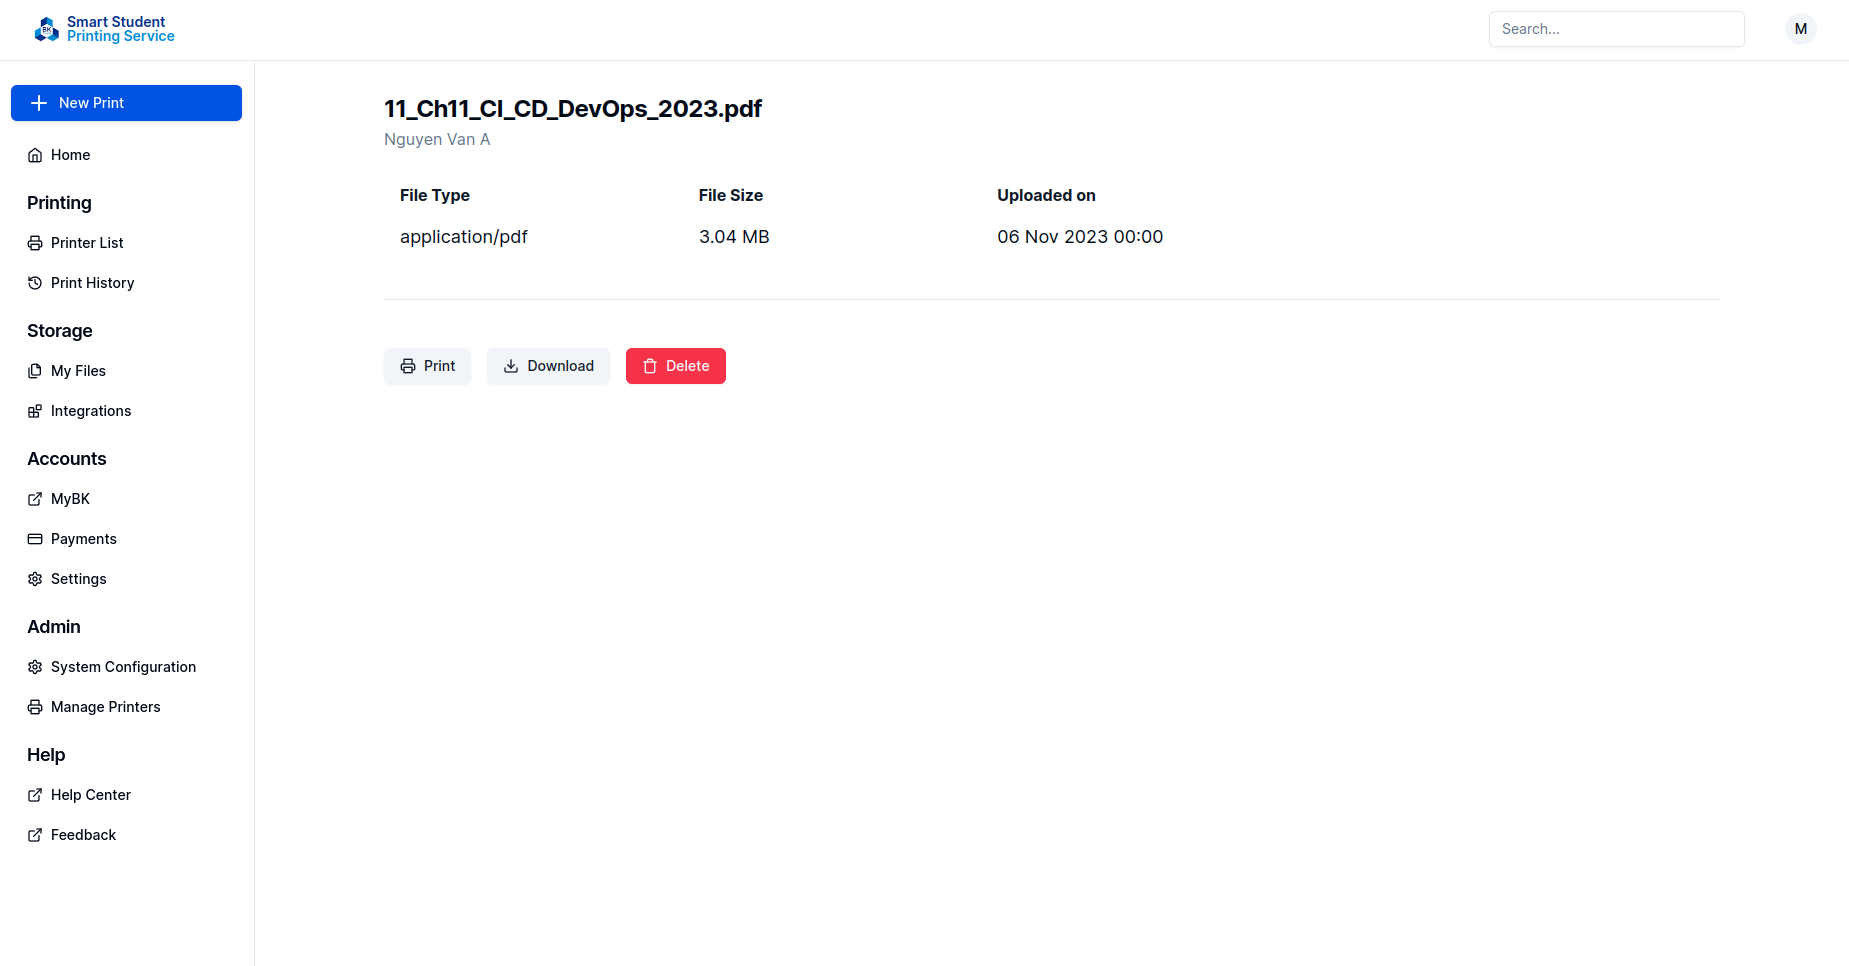
\includegraphics[max width = 0.9\linewidth,origin = c]{chapters/8. Implementation - Sprint 2/9. files - details.png}
    \caption{File Detail Page}%
\end{figure}

\subsubsection{System Configuration}

\begin{figure}[H]
    \centering
    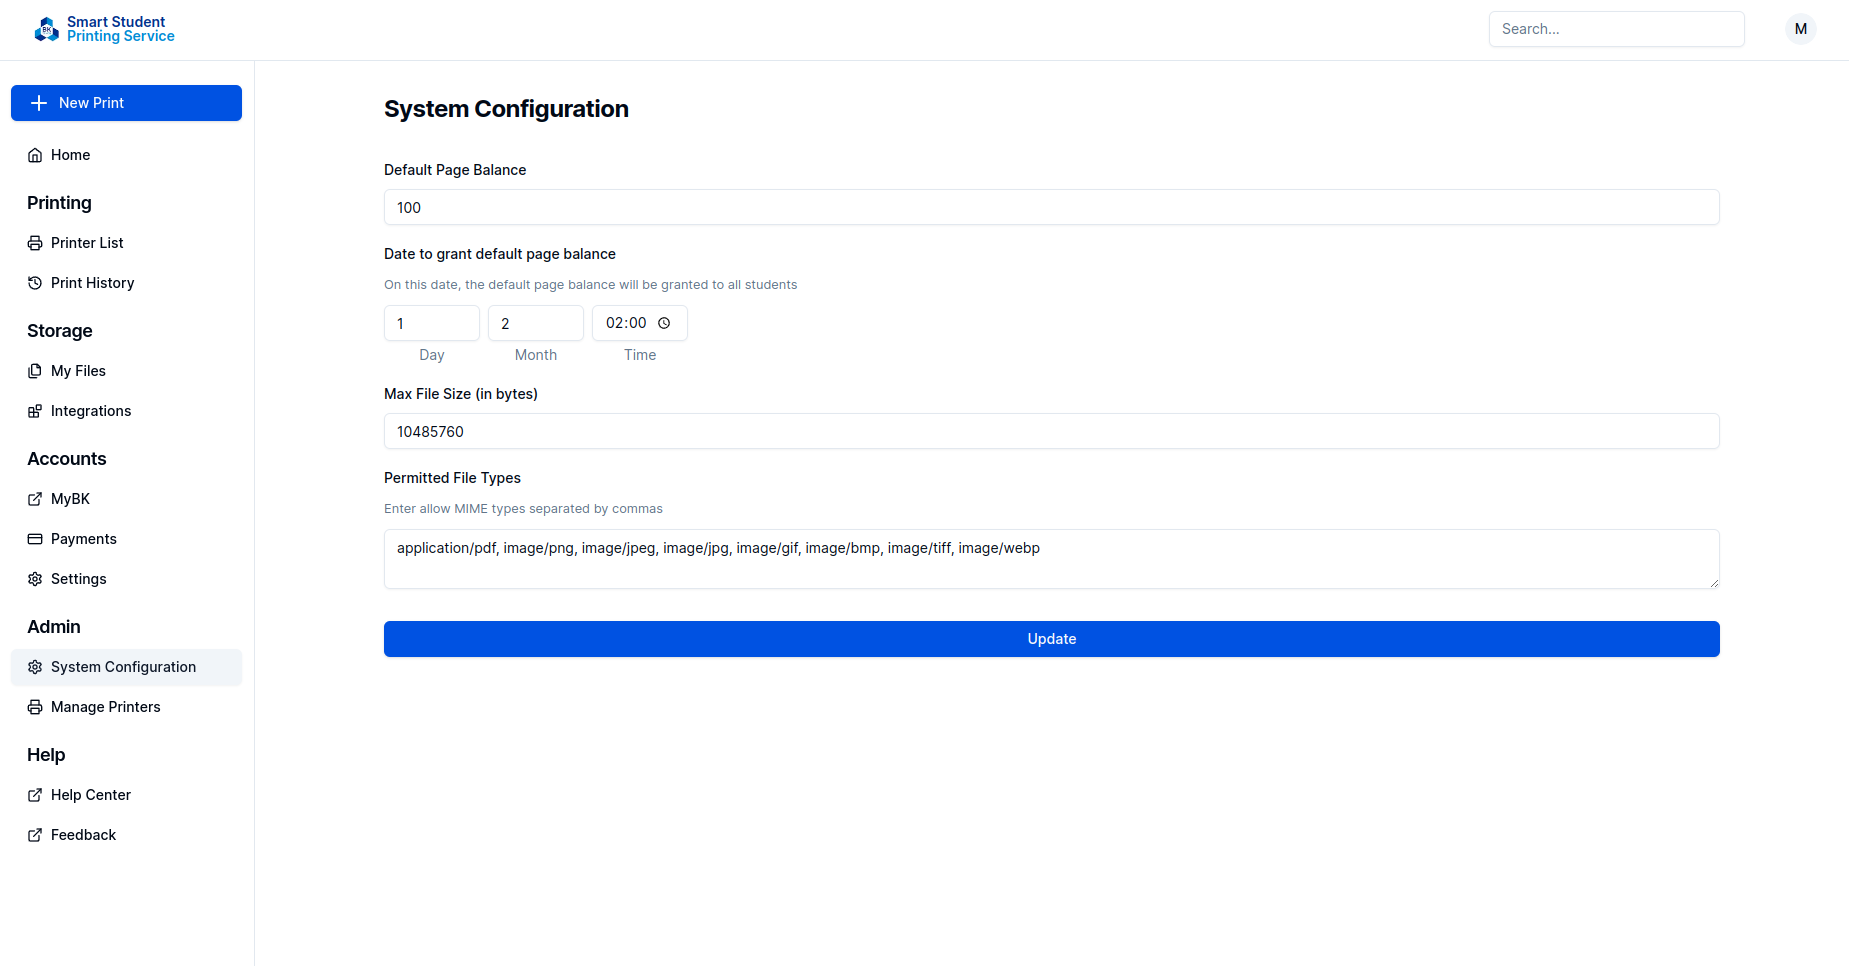
\includegraphics[max width = 0.9\linewidth,origin = c]{chapters/8. Implementation - Sprint 2/10. system configuration.png}
    \caption{System Configuration}%
\end{figure}

\subsubsection{Manage printer}

\begin{figure}[H]
    \centering
    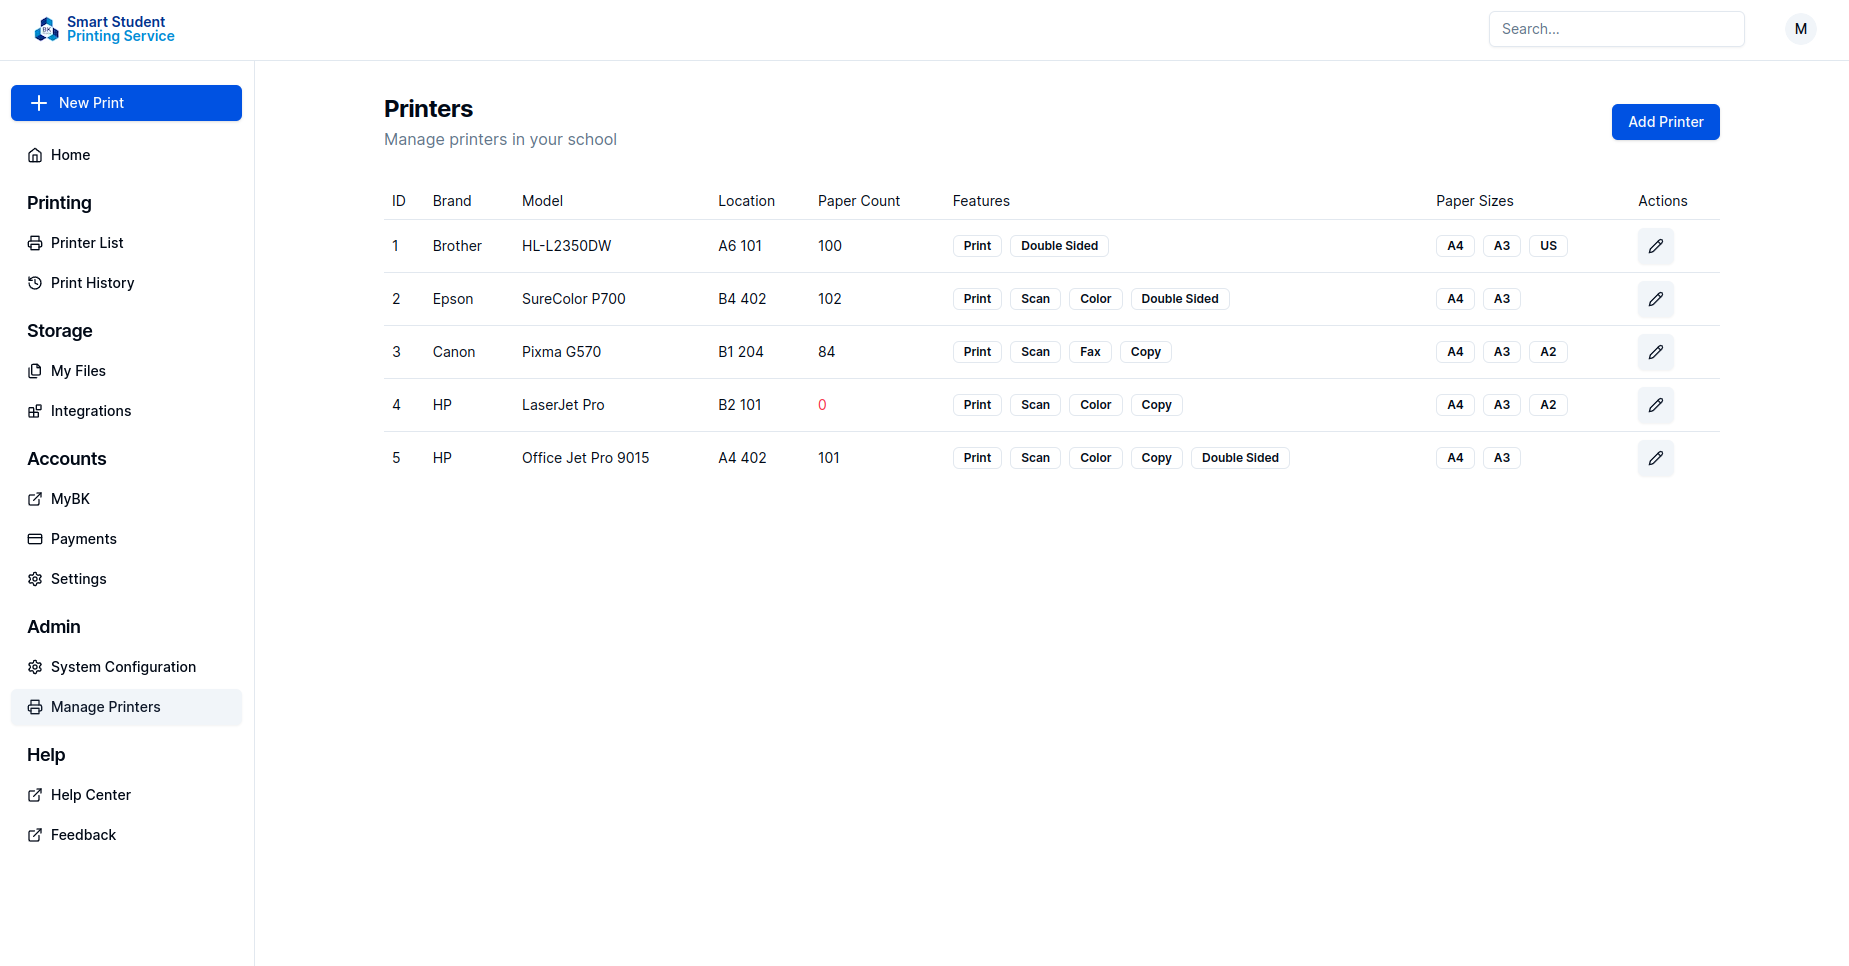
\includegraphics[max width = 0.9\linewidth,origin = c]{chapters/8. Implementation - Sprint 2/11. manage printers.png}
    \caption{Manage Printers}%
\end{figure}
\begin{figure}[H]
    \centering
    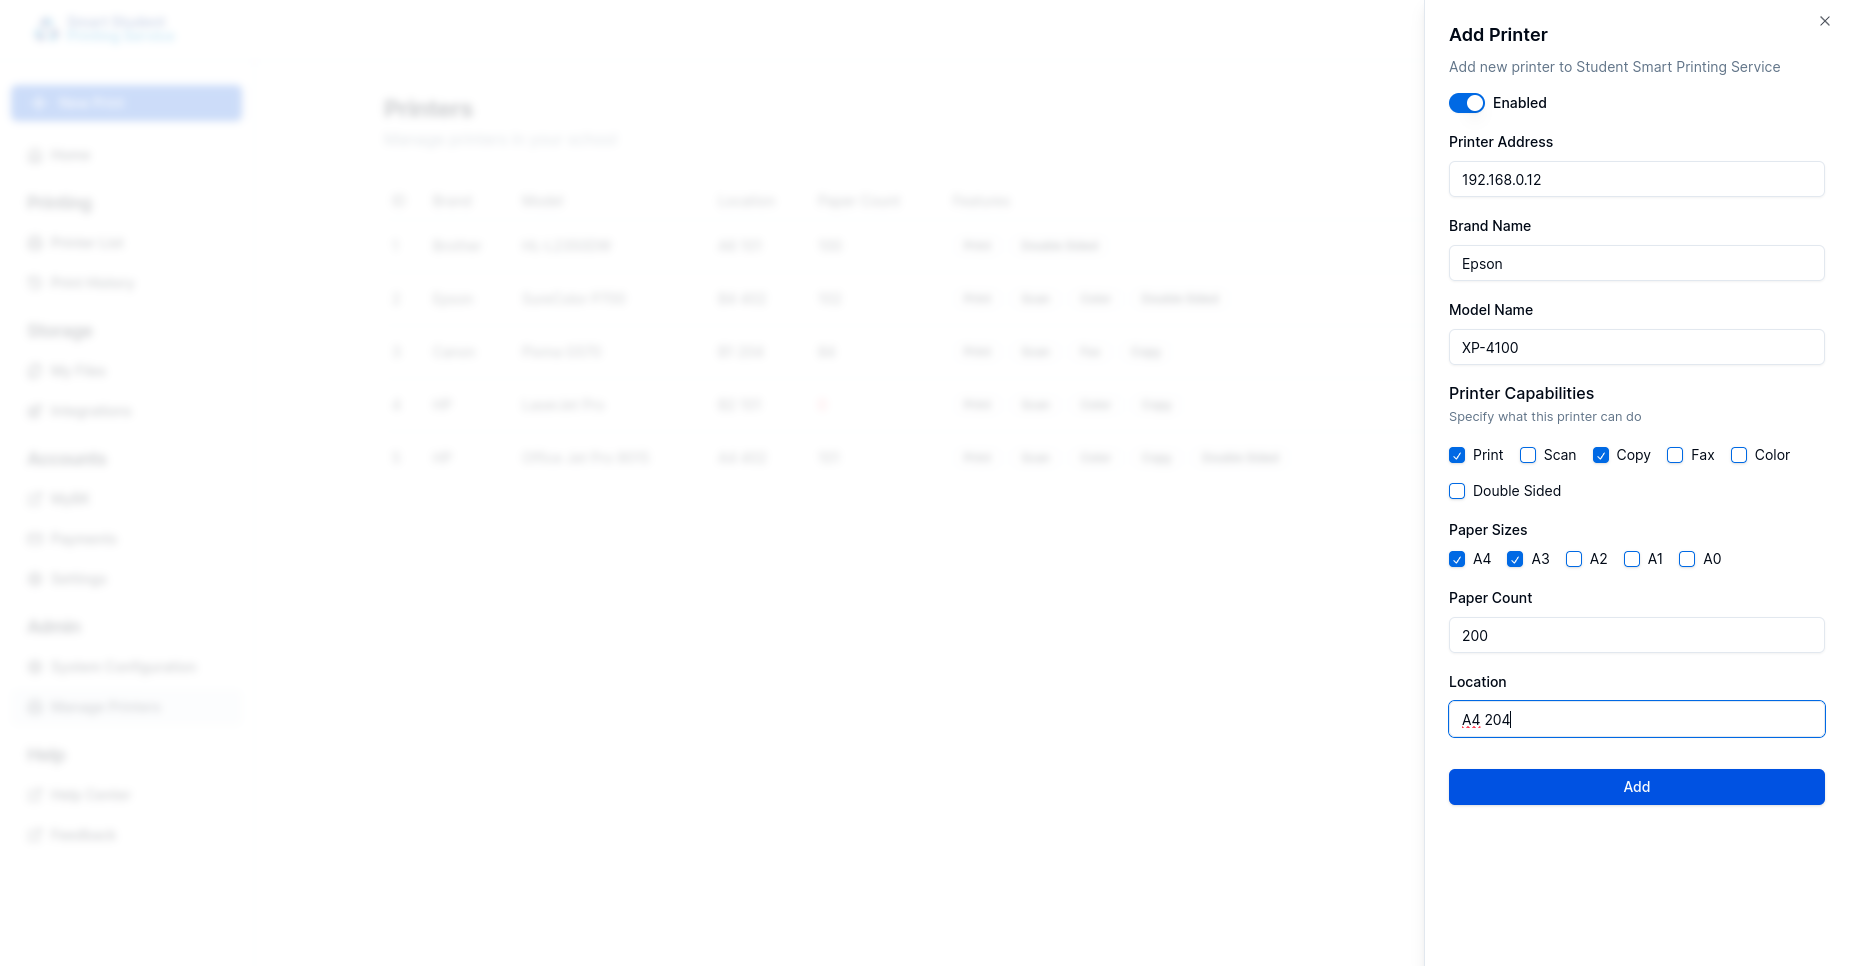
\includegraphics[max width = 0.9\linewidth,origin = c]{chapters/8. Implementation - Sprint 2/12. manage printers - form.png}
    \caption{Manage Printers - Create/Update Printer}%
\end{figure}
\clearpage

\nocite{*}

\end{document}
